%% ===================================================================
%%  Query-difficulty-conditioned retrieval control for on-device RAG
%%  Journal version. Single self-contained file: the bibliography is
%%  embedded, so there is no .bib to upload and no bibtex pass to run.
%%
%%  BUILD (Overleaf)
%%    Upload this file together with the eight figure PDFs, all in the
%%    same folder. Set the main document to journal.tex. Compile with
%%    pdfLaTeX, three times.
%%
%%  BUILD (locally)
%%    pdflatex journal && pdflatex journal && pdflatex journal
%%
%%  Needs: IEEEtran, algorithm, algpseudocode, booktabs, multirow,
%%  cite, hyperref. All are in a standard TeX Live or MiKTeX install.
%%
%%  Every quantitative claim in this manuscript is traceable to a file
%%  written by a recorded run; scripts/check_paper_numbers.py asserts
%%  the mapping and fails if any figure has drifted.
%% ===================================================================

\documentclass[journal]{IEEEtran}
%% For a double-spaced single-column submission copy, replace the line
%% above with:
%%     \documentclass[journal,onecolumn,draftclsnofoot,12pt]{IEEEtran}
%% Nothing else in this file needs to change.

\usepackage{cite}
\usepackage{amsmath,amssymb,amsfonts}
\usepackage{algorithm}
\usepackage{algpseudocode}
\usepackage{graphicx}
\usepackage{booktabs}
\usepackage{multirow}
\usepackage{array}
\usepackage{url}
\usepackage{textcomp}
\usepackage[hidelinks]{hyperref}

%% The figures sit beside this file on Overleaf, and under results/paper/
%% in the repository. Both locations are searched, so the same file
%% compiles in either place.
\graphicspath{{./}{../results/paper/}}

\newcommand{\nprobe}{\texttt{nprobe}}
\newcommand{\degC}{\,^{\circ}\mathrm{C}}

\begin{document}

\title{Spend effort where it buys something:
query-difficulty-conditioned retrieval control for
on-device retrieval-augmented generation}

\author{Anshuman~Kumar,
        Govind~Mukund~Agarwal,
        and~Shivam~Kumar%
\thanks{The authors are with the School of Computer Science and
Engineering, Vellore Institute of Technology, Vellore 632014, Tamil Nadu,
India (e-mail: anshuman.kumar@vitstudent.ac.in;
govind.mukund2023@vitstudent.ac.in; shivam.kumar2023c@vitstudent.ac.in).}%
\thanks{Every measurement reported in this paper, including those which
did not support the hypothesis they were collected to test, is
reproducible from the released artifact.}}

\markboth{IEEE Transactions on Mobile Computing,~Vol.~XX, No.~X, Month~20XX}%
{Kumar \MakeLowercase{\textit{et al.}}: Query-difficulty-conditioned retrieval control for on-device RAG}

\maketitle

\begin{abstract}
Retrieval-augmented generation (RAG) on a handset runs on a fixed battery
inside a chassis with no fan, so a millisecond of retrieval is heat and
charge which cannot be recovered. Published mobile RAG indexes fix their
search parameters when the index is built, and therefore spend the same
effort on every query, whether or not that effort returns anything. We
observe that the information needed to spend effort unevenly is already
computed by such an index and then discarded. A two-phase disk-resident
inverted-file index must search a resident centroid structure before it
can decide which on-disk clusters to open, and that search yields, at no
additional cost and before any expensive work is committed, a measure of
how decisively one cluster won: the gap $g = d_2 - d_1$ between the
distances to the nearest and the second-nearest centroid. Let $B$ be a
set of difficulty buckets with weights $w_b$, $L$ a set of effort levels
with handset-measured costs $c_\ell$, and $r_{b\ell}$ the measured recall
of bucket $b$ at level $\ell$. We allocate effort by maximizing
$\sum_b w_b r_{b\ell(b)}$ subject to $\sum_b w_b c_{\ell(b)} \le C$,
which for $|B| = |L| = 5$ we solve exactly by enumeration. On a
$46\,369$-passage SQuAD index we show that $g$ separates recall@$10$ at
the cheapest effort level from $0.278$ for the hardest quintile of queries
to $0.978$ for the easiest, a spread of $3.5\times$, and that one step of
additional effort is worth $+0.403$ recall to the hardest fifth and
$+0.009$ to the easiest, a difference of $45\times$. Scored on $500$
queries never used for fitting, the allocation improves recall@$10$ at
near-equal device cost on three of five budgets, by up to $+0.0162$
against a stated resolution floor of $0.0002$. We also report a negative
result. Across six recorded handset runs the sensor which Android exposes
as skin temperature never reached the $42\degC$ threshold at which our
thermal policy derates, while the hottest internal zone on the same device
exceeded it in all six, peaking at $78.8\degC$ against a skin peak of
$37.5\degC$; replaying one trace through the same policy and changing only
the sensor it reads moves the controller from full effort on $97\%$ of the
run to the floor level on $100\%$ of it. Finally we measure, rather than
extrapolate, per-query energy: $130.99$~mJ per query all-in and a marginal
$3.21$~mJ per cluster opened over $9\,670$ queries on an unplugged handset,
with median power rising $97.6\%$ from the quietest to the busiest quintile
of retrieval work.
\end{abstract}

\begin{IEEEkeywords}
On-device retrieval, retrieval-augmented generation, approximate nearest
neighbor search, inverted-file index, adaptive control, query difficulty,
energy efficiency, thermal management, mobile systems, reproducible
measurement.
\end{IEEEkeywords}

\section*{Nomenclature}
\noindent
\begin{tabular}{@{}ll@{}}
$N$ & Number of indexed passage vectors ($46\,369$).\\
$N_c$ & Number of IVF clusters ($215$).\\
$d$ & Embedding dimension ($384$).\\
$k$ & Number of neighbours returned ($10$ unless stated).\\
$\ell$ & An effort level, that is, a value of \nprobe.\\
$L$ & The set of effort levels, $\{1,4,8,16,32\}$.\\
$c_\ell$ & Handset-measured p95 latency of level $\ell$, in ms.\\
$d_1,d_2$ & Distance to the nearest, second-nearest centroid.\\
$g$ & Difficulty signal, $g = d_2 - d_1$.\\
$B$ & The set of difficulty buckets, quintiles of $g$.\\
$w_b$ & Population weight of bucket $b$.\\
$r_{b\ell}$ & Measured mean recall@$k$ of bucket $b$ at level $\ell$.\\
$C$ & Declared cost budget, in ms per query.\\
$\tau$ & Thermal time constant of the handset ($67.9$~s).\\
$\varepsilon$ & Recall resolution floor, $1/(n_{\mathrm{test}}k)$.\\
\end{tabular}

\section{Introduction}

\IEEEPARstart{R}{etrieval}-augmented generation conditions a language model
on passages fetched at inference time, so that what the model says is
grounded in a corpus and not only in its own
parameters~\cite{lewis2020rag,karpukhin2020dpr,gao2023ragsurvey}. For
personal data the attraction of this architecture is obvious. The corpus
is the user's own messages, notes and documents, and the natural place to
keep that corpus is the device which produced it. Running the whole
pipeline on the handset removes the need to upload anything, keeps the
feature working without connectivity, and removes the per-query serving
cost an operator would otherwise carry.

It also changes the cost model, in a way which the retrieval literature
largely does not account for. A datacenter retrieval system trades latency
against accuracy on the assumption that power is bought rather than stored,
and that heat is removed by infrastructure built to remove it. A phone
trades latency, accuracy, \emph{heat} and \emph{charge} at the same time,
against a battery which will not refill during the session and a passively
cooled chassis whose only response to sustained load is to grow hotter
until firmware intervenes. The environmental argument about the energy
cost of language technology has mostly been made at the scale of training
runs~\cite{strubell2019energy,schwartz2020greenai}; on a handset the same
argument applies per query, against a budget the user can watch draining.
Recent measurement studies of on-device inference make the point
concretely. Sustained workloads on phones are limited less by arithmetic
throughput than by thermal headroom, power floors and memory
bandwidth~\cite{tummalapalli2026edgeinference,cai2026npuready}, and the
relation between configuration and energy is not even
monotone~\cite{ehsani2026sustainability}.

\textbf{The inefficiency we attack.} MobileRAG~\cite{park2025mobilerag} is
the current reference design for this setting, and its EcoVector index has
the right shape for a phone: a hierarchical navigable small world (HNSW)
graph over inverted-file centroids stays resident in RAM, while each
cluster's vectors live on disk and are touched only if the search decides
to open them. A query therefore pays for the clusters it opens and for
nothing else. EdgeRAG~\cite{seemakhupt2024edgerag} arrives at a similar
structure from a different direction, generating second-level embeddings
online rather than storing them, and a wave of systems during 2025 and 2026
has continued to compress what the index must
hold~\cite{wang2025leann,killingback2026unified} and to cache what has
already been computed~\cite{liu2026percache}.

What none of these designs does is decide, per query, \emph{how hard to
look}. The search parameters, chiefly \nprobe, the number of clusters
opened, are chosen when the index is built and are then applied uniformly.
Every query receives the same effort, whether that effort was necessary or
wasted, and whether the device is cool and charging or hot and nearly flat.

Uniform allocation would be defensible provided the cost--recall curve were
close to linear, because a unit of effort would then be worth roughly the
same wherever it was spent. It is not close to linear. Fig.~\ref{fig:effort}
plots our handset-measured cost against recall: moving from one cluster to
four costs $38$~ms and buys $0.20$ recall, while moving from sixteen
clusters to thirty-two costs $164$~ms and buys $0.03$. The curve is steep
at one end and almost flat at the other, which is precisely the condition
under which \emph{who receives the effort} matters more than \emph{how much
effort there is in total}.

\textbf{The observation.} Our central observation is structural rather than
algorithmic, and this is why the method costs nothing to deploy. A
two-phase index has, by construction, a decision point between a cheap
phase and an expensive one. The cheap phase, which searches the resident
centroid structure, must run before the expensive phase can begin, because
its output is what tells the expensive phase where to look. That output
contains more than the system currently uses. It contains not only the
ranked list of candidate clusters but the \emph{distances} to them, and in
particular how far the second-best cluster sits behind the best.

A large gap means one cluster won decisively, so the true neighbours are
probably concentrated inside it and a cheap search will find them. A gap
near zero means the query fell between clusters, its neighbours are
scattered across them, and a cheap search will miss most of them. The
quantity is computed whether or not anyone reads it, it is available before
a single byte of cluster data is touched, it adds nothing to the resident
structure, and it requires no training. We show that it predicts query
difficulty well enough to beat uniform allocation at matched device cost.

\textbf{Summary of results.} As an illustration of the mechanism, in this
paper we make an analysis of one index on one handset, providing the
following results.

\begin{itemize}
\item Table~\ref{tab:separation} gives the recall of every difficulty
quintile at every effort level, and is the empirical object on which the
rest of the method rests. The quintiles separate by a factor of $3.5$ at
the cheapest level, and the marginal value of one step of effort differs
between them by a factor of $45$ (Section~\ref{sec:signal}).
\item Table~\ref{tab:alloc} gives the held-out comparison of the fitted
allocation against uniform effort. Three of five budgets improve, by $45$
to $81$ times the stated resolution floor, at near-equal device cost
(Section~\ref{sec:alloc}). Table~\ref{tab:assignments} gives the
assignment which produced each of those numbers.
\item Table~\ref{tab:profile} gives the profile table the controller
chooses from, and Table~\ref{tab:costmodel} gives the analytic cost model
we fitted and did not deploy (Section~\ref{sec:design}).
\item Fig.~\ref{fig:sensors} and Fig.~\ref{fig:trace} give the negative
result on thermal sensor selection, across every handset run we recorded
(Section~\ref{sec:sensors}).
\item Table~\ref{tab:energy} and Fig.~\ref{fig:energy} give per-query
energy and the rise of median power with retrieval work, measured on an
unplugged handset (Section~\ref{sec:energy}).
\item Table~\ref{tab:regime} gives a four-point sweep in which per-cluster
graphs cut distance computations at matched recall and lose on wall-clock
at every point, which is the measurement which forced the controller to
read a table of observed latencies rather than any model
(Section~\ref{sec:regime}).
\end{itemize}

To our knowledge this is the first use of a probe-time difficulty signal to
allocate approximate nearest neighbor (ANN) search effort under a
device-measured cost budget on a mobile index. The closest prior work either
adapts the RAG strategy above the index rather than the search effort inside
it~\cite{jeong2024adaptiverag}, or adapts inside the index but as a
\emph{stopping} rule evaluated during
search~\cite{li2020earlytermination,chatzakis2026darth} and against a server
latency objective. We discuss the first of these in
Section~\ref{sec:rel-adaptive-rag} and the second in
Section~\ref{sec:related}.

\textbf{Organization.} Section~\ref{sec:background} gives the background on
two-phase indexes and states the constraints the handset adds.
Section~\ref{sec:related} positions the work against four adjacent
literatures. Section~\ref{sec:problem} formalizes the control problem and
Section~\ref{sec:design} describes the system which implements it.
Section~\ref{sec:method} states the measurement discipline, which is needed
to judge Section~\ref{sec:sensors} and which changed our results twice.
Section~\ref{sec:signal} characterizes the difficulty signal and
Section~\ref{sec:alloc} the allocation built on it.
Section~\ref{sec:eval} evaluates the surrounding control layer.
Section~\ref{sec:sensors} reports the thermal negative result,
Section~\ref{sec:discussion} discusses when the method transfers,
Section~\ref{sec:threats} states the threats to validity, and
Section~\ref{sec:repro} describes the artifact. Section~\ref{sec:conclusion}
concludes and gives open questions.

\begin{figure*}[!t]
\centering
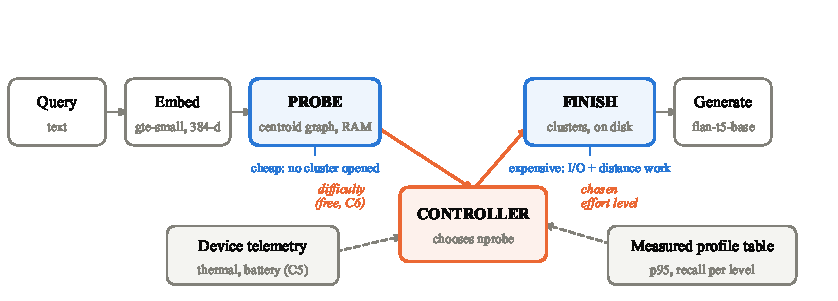
\includegraphics[width=\textwidth]{fig1_architecture.pdf}
\caption{The pipeline and the points at which each control signal enters.
The probe phase searches the centroid graph and opens no clusters; the
finish phase pays the I/O and distance cost. The controller sits between
the two. The difficulty signal of Section~\ref{sec:signal} is a by-product
of the cheap phase and is available before the expensive phase commits;
the device telemetry of Section~\ref{sec:sensors} enters at the same
point.}
\label{fig:arch}
\end{figure*}

\section{Background}
\label{sec:background}

\textbf{Inverted-file indexes and the two-phase structure.} An
inverted-file (IVF) index partitions a corpus of $N$ vectors into $N_c$
clusters, each with a centroid, and answers a query by identifying the
\nprobe{} nearest centroids and scanning only the vectors assigned to
them~\cite{johnson2021faiss,douze2024faiss}. Recall is traded against work
through \nprobe. At $\nprobe = N_c$ the search is exhaustive and exact,
and at $\nprobe = 1$ it examines roughly $N/N_c$ vectors and misses any
neighbour which fell into another partition.

Graph indexes such as HNSW~\cite{malkov2020hnsw} obtain better recall per
distance computation, but they require the graph to be resident, which is
exactly the resource a phone cannot spare. Disk-resident hybrids combine
the two ideas, in that a small structure in memory decides where to look
and the bulk stays on storage. DiskANN~\cite{subramanya2019diskann} and
SPANN~\cite{chen2021spann} established the pattern for servers with SSDs,
and EcoVector~\cite{park2025mobilerag} adapts it to handsets. Our index
follows EcoVector: an HNSW graph over $N_c = 215$ centroids in RAM, with
each cluster's vectors memory-mapped from its own file. Recall against
latency on such indexes is conventionally reported as a curve rather than
as a single point~\cite{aumuller2020annbench}, and
Section~\ref{sec:signal} argues that the asymmetry of that curve is itself
the opportunity.

The consequence which matters here is structural. Because the design is
two-phase, there exists a decision point between a cheap phase and an
expensive one, at which the system knows something about the query and has
not yet spent anything substantial on it. Single-phase designs, a flat scan
or a pure graph traversal, have no such point. A graph search can be
stopped early, which is a different and complementary
mechanism~\cite{li2020earlytermination,chatzakis2026darth}, but it cannot
be \emph{budgeted} in advance from a signal it has not yet computed. The
mechanism we describe is therefore specific to the two-phase family rather
than general to ANN search, and we state that limitation plainly because
it bounds the claim.

\textbf{What the phone adds to the objective.} Three constraints
distinguish the handset from the server, and each of them appears somewhere
in our control law.

\emph{Charge is finite and is not replenished.} Energy spent on retrieval
is energy unavailable to the rest of the session. Section~\ref{sec:energy}
quantifies the per-query figure on our device, and shows that although it
is dominated by a fixed component it has a real marginal term which effort
control can address.

\emph{Heat accumulates and is removed slowly.} The handset has no fan. Our
fitted first-order thermal model gives a time constant of $\tau = 67.9$~s
(Section~\ref{sec:method}), which is three to four orders of magnitude
longer than a single retrieval. A controller which reacts to thermal state
per query is therefore acting on observation noise, and
Section~\ref{sec:policies} shows an additive-increase multiplicative-decrease
(AIMD) controller doing exactly that.

\emph{Interactive latency targets are deadlines, not averages.} A retrieval
which takes four times its budget is not four times worse; it is a visible
stall. We therefore report the fraction of queries over budget as a
first-class quantity beside mean recall, and we do not permit any policy to
raise effort above a declared budget in the service of some other goal
(Section~\ref{sec:design}).

EdgeRAG~\cite{seemakhupt2024edgerag} is the closest system to ours in
intent, but its evaluation platform is a Jetson Orin, an embedded GPU board
with a heatsink and wall power. That difference is the reason thermal state
and charge enter our control law at all, and the reason our costs come from
a phone rather than from a board.

\section{Related work}
\label{sec:related}

We position this work against four literatures: adaptive search inside ANN
indexes, adaptive retrieval strategy above the index, on-device and edge
RAG systems, and resource-aware mobile inference.
Table~\ref{tab:positioning} summarizes the comparison on the three axes we
consider decisive, namely what is being adapted, what the adaptation signal
costs, and what the cost axis is denominated in.

\begin{table*}[!t]
\caption{Positioning against the closest prior work. The three right-hand
columns are the axes on which we claim the difference is material.}
\label{tab:positioning}
\centering
\begin{tabular}{llllll}
\toprule
System & Setting & Adapted quantity & Decision time & Signal cost & Cost axis \\
\midrule
Adaptive-RAG~\cite{jeong2024adaptiverag} & server RAG & \# retrieval/LLM calls & before retrieval & trained classifier & LLM calls \\
Self-RAG~\cite{asai2024selfrag} & server RAG & whether to retrieve & during generation & fine-tuned LM & answer quality \\
FLARE~\cite{jiang2023flare} & server RAG & when to retrieve & during generation & LM confidence & answer quality \\
Li et al.~\cite{li2020earlytermination} & server ANN & when to stop & during search & learned predictor & server latency \\
DARTH~\cite{chatzakis2026darth} & server ANN & when to stop & during search & intermediate state & server latency \\
Quake~\cite{mohoney2025quake} & server ANN & index structure & background & maintenance cost & query/update latency \\
KScaNN~\cite{senkevich2025kscann} & server ANN & \nprobe{} & before search & learned predictor & server throughput \\
EdgeRAG~\cite{seemakhupt2024edgerag} & edge board & embedding generation & during search & profiling & board latency \\
MobileRAG~\cite{park2025mobilerag} & handset & fixed at build time & --- & --- & analytic distance count \\
\textbf{This work} & \textbf{handset} & \textbf{\nprobe{} per query} & \textbf{before finish phase} & \textbf{free by-product} & \textbf{measured ms and mJ} \\
\bottomrule
\end{tabular}
\end{table*}

\subsection{Adaptive search inside the index}

Adaptivity in ANN search is not new. Li et al.~\cite{li2020earlytermination}
learn to terminate graph search early on a per-query basis, predicting from
intermediate search state when further exploration will not improve the
result. Our approach differs in two ways which matter for the mobile
setting. First, their signal is observed \emph{during} search, which makes
the decision a stopping rule, whereas ours is observed \emph{before} the
expensive phase, from the output of the probe, which makes the decision a
budgeting rule: the work is never started rather than started and
abandoned. Second, and more important for a phone, their objective is
latency on a server, whereas ours is allocation against a table of
latencies measured on the target handset, so that the optimizer trades
recall against milliseconds which were actually observed on the device
which will run the query.

DARTH~\cite{chatzakis2026darth} makes the case for adaptivity more sharply
still, and from the premise we also start from, that a single fixed
parameter setting gives good recall on some queries and poor recall on hard
ones, so that a declarative recall target is better served by terminating
per query; the reported speedups average $6.8\times$ to $13.6\times$ across
index types. The distinction from our work is again \emph{when} the
decision is taken. DARTH decides when to stop once search is under way; we
decide what to spend before it starts. The two are compatible, in that a
budget chosen from difficulty could then be terminated early by a recall
target, and we regard that composition as the natural next step rather than
as a competing design.

Two systems from 2025 are closer still on the specific lever.
KScaNN~\cite{senkevich2025kscann} includes an adaptive predictor for the
probing count, and Quake~\cite{mohoney2025quake} adapts the index structure
itself to a shifting query distribution, reporting query latency reductions
of $1.5\times$ to $38\times$. Both target server-class hardware, both are
willing to pay for a learned or a maintained component, and neither is
evaluated against a cost axis denominated in device-measured energy. Recent
work on graph hardness~\cite{hua2026hardness} independently confirms the
premise that query difficulty is the right conditioning variable,
introducing an escape hardness metric for out-of-distribution queries; it
operates on graph geometry during search rather than on a probe-time
by-product, so it is complementary to, rather than overlapping with, the
signal we use.

Anisotropic quantization~\cite{guo2020scann} and related work improve the
accuracy per byte of the index itself. That direction is orthogonal to
ours: a better index changes the numbers in the profile table our
controller reads, and the controller keeps working unmodified.

\subsection{Adaptive retrieval strategy above the index}
\label{sec:rel-adaptive-rag}

A parallel line of work adapts the \emph{RAG strategy} rather than the
search inside it. Adaptive-RAG~\cite{jeong2024adaptiverag} is the closest
prior work in spirit, in that it routes each question to no retrieval,
single-step retrieval or iterative retrieval according to a predicted
complexity class. Self-RAG~\cite{asai2024selfrag} has the model itself
decide when to retrieve and critique what it retrieved,
FLARE~\cite{jiang2023flare} triggers retrieval mid-generation when the
model's own confidence drops, and Mallen et al.~\cite{mallen2023whennot}
show that retrieval helps unevenly across questions, which is the empirical
premise all of these rest on.

Our work differs from this line on three axes, the first of which we
consider decisive.

\emph{The lever.} These systems choose how many \emph{LLM and retrieval
calls} to make. We choose how much \emph{ANN search effort} to spend inside
a single retrieval, that is, how many clusters to open. The two are
orthogonal: an Adaptive-RAG router could sit above our controller, and
every query it routed to retrieval would still face the question of how
hard to search.

\emph{The cost of the signal.} The complexity classifier of Adaptive-RAG is
a trained model with its own training data and its own inference cost on
the query path. Our signal is a by-product of work the index performs
regardless, costs nothing additional, and requires no training. On a device
where the forward pass of a classifier would be a measurable fraction of
the budget it is trying to manage, that difference is not a detail.

\emph{The cost axis.} Their objective is answer quality against LLM calls.
Ours is recall against milliseconds and joules measured on the handset
which will run the query.

\subsection{On-device and edge RAG systems}

The systems literature for RAG outside the datacenter has grown quickly.
MobileRAG~\cite{park2025mobilerag} and EdgeRAG~\cite{seemakhupt2024edgerag}
define the two-phase shape we build on. LEANN~\cite{wang2025leann} attacks
the storage axis, recomputing embeddings on the fly rather than storing
them and reporting index size reductions up to $50\times$, and the unified
representation of Killingback et al.~\cite{killingback2026unified}
compresses the context and the retrieval representation jointly for
on-device use. PerCache~\cite{liu2026percache} caches and predicts across
queries, reporting a $34.4\%$ latency reduction on mobile RAG, and Feric et
al.~\cite{feric2026adaptivecompression} apply telemetry-guided adaptive
compression to the retrieved context on edge devices, reporting energy
savings up to $53\%$. Ren et al.~\cite{ren2024mec} consider RAG in a mobile
edge computing topology in which the heavy work is offloaded rather than
performed locally, and Loo et al.~\cite{loo2025mobileagent} use retrieval
to improve a mobile agent rather than to reduce its cost.

All of these change \emph{what} is stored, cached, compressed or offloaded.
None of them changes \emph{how much search effort an individual query
receives}, which is the variable we control. The nearest in spirit is Feric
et al.~\cite{feric2026adaptivecompression}, which is telemetry-guided as we
are, but which acts on the context handed to the generator rather than on
the retrieval which produced it. The two compose cleanly, and
Section~\ref{sec:joint} reports what happens when we sweep our own
reduction mechanism jointly with retrieval effort.

\subsection{Resource-aware mobile inference}

Thermal and energy management for on-device inference is an active area
whose standard levers are dynamic voltage and frequency scaling, model
switching and tier routing. Benchmarking infrastructure for the setting has
matured. MELT~\cite{laskaridis2024melt} traces language-model workloads on
real handsets at fine granularity, covering performance, energy and thermal
behaviour together, and the AI Benchmark series~\cite{ignatov2019aibench}
established the practice of reporting smartphone inference across devices
rather than on one. More recently, EnerInfer~\cite{zou2026enerinfer} shows
that modestly lowering NPU and memory frequencies preserves quality of
experience while substantially improving energy efficiency, using
limited-horizon thermal prediction to switch regimes;
ThermE~\cite{lu2026therme} manages shared thermal headroom predictively for
sustained inference on thermally constrained edge SoCs; and Cai et
al.~\cite{cai2026npuready} instrument mobile power telemetry directly, to
expose efficiency bottlenecks which framework-level timing hides.

Our measurement apparatus (Section~\ref{sec:method}) belongs to this
tradition, applied to retrieval rather than to generation. Our negative
result (Section~\ref{sec:sensors}) is, we believe, a useful contribution
back to it. The systems above take a thermal signal as given, and we show
that on a consumer handset the choice of which thermal signal to read
dominates the choice of threshold by tens of degrees.

We are not aware of prior work which treats \emph{retrieval effort} as the
controlled variable on a phone, with the control law reading device
telemetry. Section~\ref{sec:sensors} reports what happened when we tried,
including why the thermal half of it did not work.

\section{The control problem}
\label{sec:problem}

\textbf{Setting.} Let $\mathcal{X} = \{x_1,\dots,x_N\} \subset
\mathbb{R}^{d}$ be the indexed passage embeddings, L2-normalized and
searched under inner product, let $\mathcal{C} = \{c_1,\dots,c_{N_c}\}$ be
the IVF centroids, and let $P : \mathcal{X} \to \mathcal{C}$ be the
assignment of vectors to clusters. For a query embedding $q$, write the
centroids in order of increasing distance as $c_{(1)}, c_{(2)}, \dots$ and
let $d_i = \delta(q, c_{(i)})$, where $\delta(u,v) = 1 - \langle u,
v\rangle$.

A retrieval at effort level $\ell$ returns the $k$ nearest vectors found
among the clusters of $c_{(1)},\dots,c_{(\ell)}$. Let $G_k(q)$ be the true
$k$ nearest neighbours of $q$ in $\mathcal{X}$, and let $R_k(q,\ell)$ be
the returned set. Recall is
\begin{equation}
\mathrm{rec}(q,\ell) = \frac{|R_k(q,\ell) \cap G_k(q)|}{k}.
\label{eq:recall}
\end{equation}

\textbf{The decision.} For each query the controller observes a feature
vector which is available \emph{before} the finish phase commits, and must
emit a level $\ell \in L$. In our instantiation that feature vector is
one-dimensional, namely the probe-time gap $g$ of~(\ref{eq:gap}). Writing
$\pi$ for the policy, the objective over a query population $Q$ is
\begin{equation}
\max_{\pi}\ \mathbb{E}_{q \sim Q}\big[\mathrm{rec}(q, \pi(q))\big]
\quad\text{s.t.}\quad
\mathbb{E}_{q \sim Q}\big[c_{\pi(q)}\big] \le C ,
\label{eq:objective}
\end{equation}
where $c_\ell$ is the cost of level $\ell$ \emph{as measured on the target
device}, and not as predicted by a model. Section~\ref{sec:design} explains
why that distinction is load-bearing and Section~\ref{sec:regime} shows
what goes wrong when it is not respected.

Two features of~(\ref{eq:objective}) are worth noting. The constraint is on
the \emph{expectation} of cost and not on the cost of each query, which is
what permits reallocation at all, since some queries may exceed the
per-query budget provided others fall below it. And the problem is trivial
if $\mathrm{rec}$ does not depend on $q$ beyond its level, because if every
query gained the same recall from the same effort then every feasible
policy with the same mean cost would score identically. The whole method
therefore rests on an empirical question: does any cheaply observable
feature of $q$ predict $\mathrm{rec}(q,\ell)$? Section~\ref{sec:signal}
answers it.

\textbf{Reduction to a bucketed assignment.} Solving~(\ref{eq:objective})
over arbitrary measurable policies is neither necessary nor desirable on a
device. We restrict $\pi$ to depend on $q$ only through a bucket index
$b(q) \in B$, where the buckets are quantiles of the observed distribution
of $g$. This yields a finite problem, one level per bucket, and buys three
practical properties. The policy is a lookup table of $|B|$ entries, so
that its runtime cost is a comparison chain and not an inference pass. The
bucket edges are derived from data rather than chosen by hand, so that no
threshold has to be justified. And the search space is small enough to
enumerate exactly, so that the optimum is not conditional on the tolerance
of a solver. Section~\ref{sec:alloc} develops this and
Algorithm~\ref{alg:fit} states it procedurally.

\section{System design}
\label{sec:design}

\textbf{Index and pipeline.} Our corpus is the SQuAD~\cite{rajpurkar2016squad}
development passages, sentence-windowed into $46\,369$ chunks and embedded
to $384$ dimensions with a \texttt{gte-small} encoder~\cite{li2023gte},
L2-normalized and searched under inner product, which is the dense
single-vector retrieval setting established by DPR~\cite{karpukhin2020dpr}.
The index is built with $N_c = 215$ clusters, giving an average of $216$
vectors per cluster. Answer generation, where it is exercised, uses
\texttt{flan-t5-base}~\cite{chung2024flan} with greedy decoding.

A query proceeds as in Fig.~\ref{fig:arch}. It is embedded; the
\emph{probe} phase searches the resident centroid graph and returns the
clusters ranked by distance; the controller chooses \nprobe; the
\emph{finish} phase opens exactly that many cluster files and merges their
results by true distance; and the retrieved passages are assembled into a
prompt and generated from. The position of the controller, after the probe
and before the finish, is the whole point of the design, and is what
distinguishes a budgeting rule from a stopping rule.

\textbf{The profile table.} The controller does not predict cost from a
model. It chooses from a table of \emph{measured} costs, one row per effort
level, recorded on the target handset (Table~\ref{tab:profile}, plotted in
Fig.~\ref{fig:effort}). Each row is the p50 and p95 latency and the
recall@$10$ over $3\,829$ queries executed on the device.

\begin{table}[!t]
\caption{The profile table: effort levels as measured on the handset (vivo
I2304), $3\,829$ queries per level. The controller selects a row and does
not interpolate between rows. The last column is the recall purchased per
millisecond by the step which ends at that row.}
\label{tab:profile}
\centering
\begin{tabular}{rrrrr}
\toprule
\nprobe & p50 (ms) & p95 (ms) & recall@10 & $\Delta$recall / $\Delta$p95 \\
\midrule
1  & 5.59   & 13.82  & 0.6405 & --- \\
4  & 20.50  & 52.26  & 0.8417 & $5.2\times10^{-3}$ \\
8  & 40.46  & 101.46 & 0.9065 & $1.3\times10^{-3}$ \\
16 & 82.61  & 189.82 & 0.9507 & $5.0\times10^{-4}$ \\
32 & 169.21 & 354.10 & 0.9788 & $1.7\times10^{-4}$ \\
\bottomrule
\end{tabular}
\end{table}

\begin{figure}[!t]
\centering
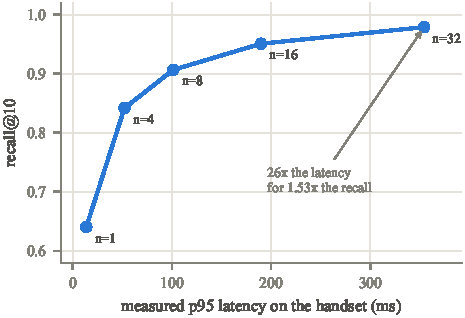
\includegraphics[width=\columnwidth]{fig2_effort_return.pdf}
\caption{The curve the controller chooses from, measured on the handset.
Each marked point is one row of Table~\ref{tab:profile}, plotted as p95
latency against recall@$10$. The annotation compares the two ends of the
curve: thirty-two clusters cost $26$ times the latency of one cluster and
return $1.53$ times the recall.}
\label{fig:effort}
\end{figure}

The last column of Table~\ref{tab:profile} makes the asymmetry arithmetic.
The recall purchased per millisecond falls by a factor of $31$ between the
first step and the last. Spending the marginal millisecond at the bottom of
the curve rather than at the top is therefore worth more than any constant
factor the implementation could plausibly recover.

We use a measured table rather than the analytic cost model we also fitted,
because that model fails exactly where it matters. Fitted on the quiet
phases of three runs ($21\,388$ samples) it reaches $14.75\%$ mean absolute
percentage error (MAPE), inside our declared $15\%$ target; held out on
contended phases it degrades to $35.87\%$. Table~\ref{tab:costmodel} gives
the per-term fit quality and shows where the error concentrates. A
predictor which is most wrong when the CPU is busiest would choose the
wrong level exactly when choosing right matters most, and so we did not
deploy it.

\begin{table}[!t]
\caption{The analytic cost model we fitted and did not deploy, fitted on
$21\,388$ samples from the quiet phases of three runs. The model is
internally sound on two of its three terms and is still unusable, for the
reason given in the text.}
\label{tab:costmodel}
\centering
\begin{tabular}{llrr}
\toprule
Term & Features & $R^2$ & MAPE (fit) \\
\midrule
$t_{\mathrm{centroid}}$ & CPU utilization & 0.001 & 11.7\% \\
$t_{\mathrm{cluster\ load}}$ & loads, bytes, CPU & 0.992 & 7.7\% \\
$t_{\mathrm{cluster\ search}}$ & distance counts, CPU & 0.987 & --- \\
\midrule
\multicolumn{2}{l}{\emph{whole model, quiet phases}} & & 14.75\% \\
\multicolumn{2}{l}{\emph{whole model, contended phases}} & & 35.87\% \\
\bottomrule
\end{tabular}
\end{table}

Two further properties of the fit are worth recording, because they are the
kind of thing the users of a cost model should be told. The coefficients on
cluster count and bytes read are \emph{weakly identified}: the two features
correlate at $r = 0.966$ in the recorded data, because the clusters in this
index are of similar size, giving a design-matrix condition number of
$4.9\times10^{6}$. Their combined effect is well determined, in that the
term reaches $R^2 = 0.992$, but the individual coefficients are unstable
and must not be interpreted separately. And the dependence of centroid
search time on the search width of the centroid graph is
\emph{unidentifiable} from our data, because that parameter was constant at
$128$ in every recorded run. We report both rather than present a
clean-looking equation.

\textbf{The policy algebra.} All policies select a row of the profile
table. They compose, and the composition rule is part of the design rather
than an implementation detail.

\begin{itemize}
\item \textsc{Static} fixes a level.
\item \textsc{Budget} selects the highest-recall row whose measured p95
fits a declared latency target, with a $0.9$ headroom factor.
\item \textsc{Aimd} adjusts multiplicatively from observed latency, in the
manner of a congestion controller.
\item \textsc{Device} composes over \textsc{Budget} and may only
\emph{lower} the level \textsc{Budget} chose, on thermal or battery
grounds.
\item \textsc{QueryAdaptive} (Section~\ref{sec:alloc}) likewise composes
over \textsc{Budget} and may only lower.
\end{itemize}

The one-directional composition rule is deliberate and it constrains our
own results. A policy able to raise effort above the budget, because it
judged a query hard or because it wanted to finish before the device got
hotter, could miss the declared latency target in the service of some other
goal. No such trade was declared by the contract of the system, and so no
policy is permitted to make it. The consequence is that
\textsc{QueryAdaptive} can only redistribute effort downward from the
budgeted level and upward within what it saves, which is a strictly harder
setting than one in which hard queries may simply be given more time.

\begin{algorithm}[!t]
\caption{Query-adaptive retrieval, runtime path}
\label{alg:runtime}
\begin{algorithmic}[1]
\Require query $q$; centroid index $H$; bucket edges $e_1 < \dots < e_{|B|-1}$;
         level table $\Lambda : B \to L$; budget level $\ell_{\max}$
\State $(\,(c_{(1)}, d_1), (c_{(2)}, d_2), \dots\,) \gets \textsc{Probe}(H, q)$
       \Comment{already required}
\State $g \gets d_2 - d_1$ \Comment{free: no new distance is computed}
\State $b \gets$ index of the interval of $(e_j)$ containing $g$
\State $\ell \gets \min\{\Lambda(b),\ \ell_{\max}\}$ \Comment{may only lower}
\State \Return $\textsc{Finish}(q, c_{(1)}, \dots, c_{(\ell)})$
\end{algorithmic}
\end{algorithm}

Algorithm~\ref{alg:runtime} gives the runtime path. Lines~2--4 are the
entire addition: one subtraction, a comparison chain of length $|B|-1$, and
a minimum. Section~\ref{sec:policies} measures the decision cost of the
controller at no more than $0.167\%$ of the query it governs.

\section{Measurement methodology}
\label{sec:method}

This section describes how we decided what we were allowed to claim. We
include it because the discipline changed our results twice, and because a
reader judging the negative result of Section~\ref{sec:sensors} needs to
know that it was not simply a run we chose not to debug. The position it
stakes out is the one which recent mobile measurement work has been
converging
on~\cite{laskaridis2024melt,cai2026npuready,ehsani2026sustainability}: on a
phone, what the software stack reports and what the hardware is doing are
different quantities, and conflating them produces confident wrong numbers.

\textbf{Absence is represented, and not defaulted.} Every telemetry field
the platform cannot supply is \texttt{NaN} and never zero. Every policy
which reads a device signal checks for finiteness and declines to act on an
absent one. The distinction is load-bearing rather than decorative. A
laptop with no thermometer and a phone sitting at $27\degC$ both produce an
empty list of reasons from the thermal policy, and reporting those two
identically would present \emph{the absence of a measurement} as \emph{a
measurement of good health}. In Section~\ref{sec:sensors} this is what
revealed that $97.3\%$ of the decisions of our thermal policy had no device
signal behind them at all, a fact which an implementation defaulting to
zero would have hidden behind a plausible-looking success.

\textbf{Derived quantities may be refused.} We fitted a first-order lumped
thermal model,
\begin{equation}
\frac{\mathrm{d}T}{\mathrm{d}t} = a\,w + b\,(T - T_{\mathrm{ref}}) + c ,
\label{eq:thermal}
\end{equation}
in which $w$ is the retrieval work rate in clusters per second, obtaining a
time constant $\tau = -1/b = 67.9$~s at $R^2 = 0.30$.

The differencing window used to estimate~(\ref{eq:thermal}) is an analysis
choice, and it moves $R^2$ by a factor of six. Reporting a single window
would hide that, and so Table~\ref{tab:thermalsweep} reports the sweep. We
select the $30$~s window, which is the best $R^2$ among the windows
retaining at least $30$ intervals. The $120$~s window scores highest and is
excluded, because eleven points against three free parameters is a number
which flatters itself. What justifies using $\tau$ at all is the last
column: the point estimates barely move across the windows even as $R^2$
swings, so that the time constant is a stable feature of the device rather
than an artifact of the window.

\begin{table}[!t]
\caption{Sensitivity of the thermal model to the differencing window. Each
row is one fit of~(\ref{eq:thermal}) at the stated window, over the
intervals that window leaves. The selected window is in bold.}
\label{tab:thermalsweep}
\centering
\begin{tabular}{rrrr}
\toprule
Window (s) & Intervals & $R^2$ & $\tau$ (s) \\
\midrule
3   & 446 & 0.109 & 107.3 \\
15  & 89  & 0.229 & 67.1 \\
\textbf{30}  & \textbf{44}  & \textbf{0.304} & \textbf{67.9} \\
60  & 22  & 0.187 & 97.1 \\
120 & 11  & 0.691 & 76.3 \\
\bottomrule
\end{tabular}
\end{table}

We use $\tau$, because a controller acting faster than the thermal
observation delay is acting on noise. We \emph{refuse} to use the same fit
to decompose a temperature rise into contributions, because the trace it
was fitted on was recorded with the handset on AC power: charger heat is
absorbed into the constant term $c$, so that $c$ is not the idle thermal
state of the device. An early version of this decomposition attributed
$+216\degC$ to retrieval on a run whose thermometer moved $5.6\degC$. The
tempting repair is to drop the offending term and keep the rest. We instead
refuse the entire decomposition and report it as refused, because a
decomposition whose residual term is known to be contaminated does not
become trustworthy by deleting the part which made the contamination
visible.

\textbf{Anything fitted is validated held out.} The allocation of
Section~\ref{sec:alloc} is fitted on one half of the query set and scored
on the other, with the split fixed by seed. Difficulty buckets fitted and
then evaluated on the same queries would measure memorization, and would
produce a real-looking number. The point generalizes: every quantity in
this paper which was chosen by looking at data is scored on data which was
not looked at.

\textbf{A resolution floor is stated.} With $n_{\mathrm{test}} = 500$
held-out queries at $k = 10$, one query gaining one neighbour moves mean
recall by exactly
\begin{equation}
\varepsilon = \frac{1}{n_{\mathrm{test}}\,k} = \frac{1}{5000} = 0.0002 .
\label{eq:floor}
\end{equation}
We report this floor beside every difference, so that a reader can see at a
glance whether an effect is an effect or four queries. We also mark
$3\varepsilon$ on Fig.~\ref{fig:alloc}(b) rather than leave the comparison
to the arithmetic of the reader.

\textbf{What is measured where.} Retrieval was executed on a physical
handset (vivo I2304). The profile table, the policy comparison of
Section~\ref{sec:sensors} and the energy measurements are all on-device,
totalling $39\,438$ recorded queries in the run used for
Section~\ref{sec:sensors} alone. Generation was \emph{not} run on the
handset; the generation timings in our pipeline are host numbers and are
labelled as such throughout.

Recall, by contrast, is a property of the index and the query rather than
of the machine. The same query at the same \nprobe{} returns the same
neighbours anywhere, because the computation is deterministic and the
floating-point reductions are performed in the same order. Recall measured
on the host therefore transfers unchanged, and we rely on that in
Sections~\ref{sec:signal} and~\ref{sec:alloc} while taking every cost from
the handset table. We state the reliance explicitly, because it is the one
place at which a host number enters a result we claim about a device.

\section{The probe-time difficulty signal}
\label{sec:signal}

\textbf{Definition.} When the probe phase searches the centroid graph it
necessarily obtains the distances to the nearest centroids. We define the
difficulty signal as the gap between the two nearest,
\begin{equation}
g = d_2 - d_1 .
\label{eq:gap}
\end{equation}

This is a difference and not the ratio $d_2/d_1$, which might look like the
more natural scale-free choice. The ratio divides by a quantity which can
be zero or negative, since for duplicate or near-duplicate vectors under
inner product on L2-normalized \texttt{float32} rows, $1 - \langle q,
c\rangle$ can land marginally below zero through rounding. The ratio is
then undefined or sign-flipped on exactly those queries, the ones sitting
almost on top of a centroid, where the signal should be most confident. The
difference carries the same ordering information over the region which
matters and is always defined, and so we use it.

The semantics are geometric. A large $g$ means one cluster won decisively,
so that the Voronoi cell containing $q$ is entered well away from its
boundary and the true neighbours are probably inside it. A small $g$ means
$q$ sits close to the bisector between two cells, so that its true
neighbours are split across them and a search which opens few clusters will
systematically miss the ones on the far side. The signal is thus a direct
measure of the quantity which causes IVF recall loss in the first place,
namely boundary effects in the partition.

Critically, $g$ costs nothing. It is a by-product of work the index must do
regardless, it is available before any cluster file is touched, it adds no
memory to the resident structure, and it requires no training data. The
contrast with a learned difficulty classifier is not that one is more
accurate but that one is free.

\textbf{The signal separates, and by a large margin.}
Table~\ref{tab:separation} is the empirical core of this paper. We bucket
$1\,000$ SQuAD queries into quintiles of measured $g$ and report mean
recall@$10$ for every bucket at every effort level; Fig.~\ref{fig:difficulty}(a)
plots the same matrix.

\begin{table}[!t]
\caption{Recall@$10$ by difficulty quintile and effort level, on $1\,000$
SQuAD queries. The bucket edges are quantiles of the measured gap
distribution, so that each bucket holds $20\%$ of the queries. The last row
is the ratio between the hardest and the easiest quintile at that level.}
\label{tab:separation}
\centering
\begin{tabular}{llrrrrr}
\toprule
\multirow{2}{*}{Bucket} & \multirow{2}{*}{gap range} & \multicolumn{5}{c}{recall@10 at \nprobe} \\
\cmidrule(lr){3-7}
 & & 1 & 4 & 8 & 16 & 32 \\
\midrule
Q1 (hardest) & 0.000--0.004 & 0.278 & 0.681 & 0.796 & 0.889 & 0.956 \\
Q2 & 0.004--0.008 & 0.383 & 0.720 & 0.831 & 0.912 & 0.963 \\
Q3 & 0.008--0.018 & 0.560 & 0.791 & 0.874 & 0.938 & 0.969 \\
Q4 & 0.018--0.033 & 0.836 & 0.927 & 0.963 & 0.976 & 0.990 \\
Q5 (easiest) & 0.033--0.085 & 0.978 & 0.987 & 0.994 & 0.997 & 0.999 \\
\midrule
\multicolumn{2}{l}{\emph{spread, hardest : easiest}} & $3.5\times$ & $1.4\times$ & $1.2\times$ & $1.1\times$ & $1.0\times$ \\
\bottomrule
\end{tabular}
\end{table}

\begin{figure*}[!t]
\centering
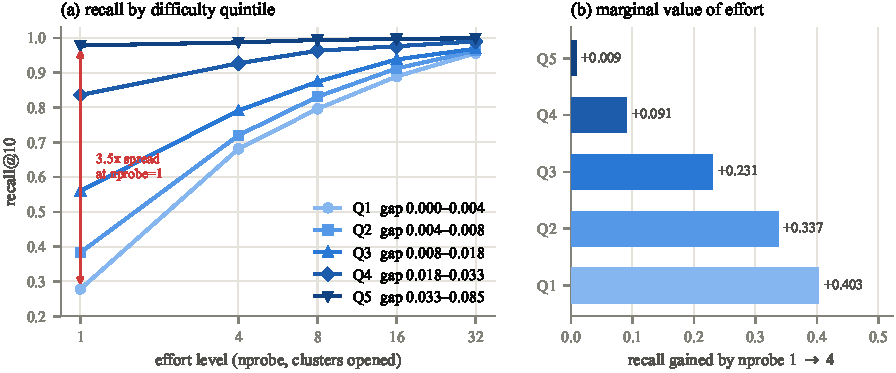
\includegraphics[width=\textwidth]{fig3_difficulty.pdf}
\caption{The observation on which the method rests, on $1\,000$ SQuAD
queries. (a) Recall@$10$ against effort, one curve per quintile of the
probe-time difficulty signal; the quintiles are ordered, and so they are
drawn as one hue stepped light to dark. The arrow marks the separation at
the cheapest level. (b) The recall gained by each quintile when effort
moves from $\nprobe = 1$ to $\nprobe = 4$, with the value of each bar
printed beside it.}
\label{fig:difficulty}
\end{figure*}

Three things in Table~\ref{tab:separation} drive everything which follows.

\emph{The separation is large at the cheap end.} At $\nprobe = 1$ the
hardest quintile recovers $0.278$ of the true neighbours and the easiest
recovers $0.978$, a spread of $3.5\times$, produced by a quantity the index
computes for free and currently discards.

\emph{The separation collapses as effort rises.} By $\nprobe = 32$ the
spread is $1.04\times$. This is not a weakness of the signal; it is the
reason the allocation has room to work only in the middle of the budget
range, and it correctly predicts the two budgets at which our allocation
cannot help (Section~\ref{sec:alloc}).

\emph{The marginal value of effort is very unequal.} Moving from $\nprobe =
1$ to $\nprobe = 4$ buys the hardest quintile $+0.403$ recall and the
easiest $+0.009$, a difference of $45\times$, plotted in
Fig.~\ref{fig:difficulty}(b). Under uniform allocation both quintiles
receive the same increment, which means that four-fifths of the step given
to Q5 is spent buying recall the query already had.

\textbf{Is the signal monotone?} A reader may reasonably ask whether the
relation is merely monotone in the aggregate or is strong enough to act on.
Two properties of Table~\ref{tab:separation} speak to this. First, recall
is monotone increasing in the bucket index at \emph{every} one of the five
effort levels, with no inversions, which is $25$ cells all ordered. Second,
the marginal gains are monotone \emph{decreasing} in the bucket index,
again with no inversions, and this is the property an allocator actually
needs, since it guarantees that moving a unit of effort from an easier
bucket to a harder one never loses on expectation. We rely on this only as
an observed regularity of this index and this corpus, and not as a theorem;
Section~\ref{sec:threats} states the corresponding threat.

\section{Effort allocation}
\label{sec:alloc}

\textbf{Fitting.} Let $B$ be the set of difficulty buckets with population
weights $w_b$, let $L$ be the set of effort levels, let $r_{b\ell}$ be the
measured mean recall of bucket $b$ at level $\ell$, and let $c_\ell$ be the
handset-measured p95 cost of level $\ell$. For a cost budget $C$ we solve
\begin{equation}
\max_{\ell : B \to L}\ \sum_{b \in B} w_b\, r_{b\,\ell(b)}
\quad \text{s.t.} \quad
\sum_{b \in B} w_b\, c_{\ell(b)} \le C .
\label{eq:alloc}
\end{equation}

Problem~(\ref{eq:alloc}) is a multiple-choice knapsack, in that each bucket
must be assigned exactly one level, the levels have costs and values, and
the total cost is bounded. In general this is NP-hard, which is why the
sizes matter. With $|B| = |L| = 5$ the space is $5^5 = 3125$ assignments,
and so we enumerate it exhaustively. The optimum is exact, the runtime is
microseconds offline, and there is no solver tolerance to defend in the
question of a reviewer. Algorithm~\ref{alg:fit} states the procedure.

\begin{algorithm}[!t]
\caption{Fitting the allocation, offline, once per index}
\label{alg:fit}
\begin{algorithmic}[1]
\Require fit queries $Q_{\mathrm{fit}}$; levels $L$; measured costs
         $\{c_\ell\}$; budget $C$; bucket count $|B|$
\For{$q \in Q_{\mathrm{fit}}$}
  \State $g(q) \gets d_2(q) - d_1(q)$ \Comment{from the probe, no extra cost}
  \For{$\ell \in L$} \State record $\mathrm{rec}(q,\ell)$ by~(\ref{eq:recall})
  \EndFor
\EndFor
\State $e_1,\dots,e_{|B|-1} \gets$ quantiles of $\{g(q)\}$ at
       $1/|B|, \dots, (|B|-1)/|B|$
\State $r_{b\ell} \gets$ mean of $\mathrm{rec}(q,\ell)$ over
       $\{q : b(q) = b\}$; \ $w_b \gets 1/|B|$
\State $\Lambda^\star \gets \arg\max$ of~(\ref{eq:alloc}) over all $|L|^{|B|}$
       assignments
\State \Return bucket edges $(e_j)$ and table $\Lambda^\star$
\end{algorithmic}
\end{algorithm}

Three properties of this formulation are deliberate.

\emph{The bucket edges are derived from data.} They are quantiles of the
measured distribution of $g$ rather than thresholds we chose, so that no
reviewer has to be persuaded that a particular cut point was not selected
after seeing the result. It also makes $w_b = 1/|B|$ by construction.

\emph{Objective and constraint are both measurements.} The quantity
$r_{b\ell}$ comes from a recall sweep and $c_\ell$ comes from the handset.
Nothing in~(\ref{eq:alloc}) is the prediction of a model, which is the
lesson that Sections~\ref{sec:design} and~\ref{sec:regime} independently
insist on.

\emph{The budget is instantiated at the cost of each uniform level.} We set
$C = c_\ell$ for each $\ell \in L$ in turn, so that every comparison
replaces a uniform policy with an allocation of the same nominal budget,
rather than comparing against whichever uniform point happens to flatter
us.

\textbf{What the allocation actually decides.}
Table~\ref{tab:assignments} gives the fitted assignment at each budget,
which we report in full because it makes the mechanism legible in a way the
aggregate differences do not.

\begin{table}[!t]
\caption{The fitted assignment at each budget: the \nprobe{} given to each
difficulty quintile, the budget $C$ it was fitted under, and the mean cost
of that assignment on the fit half.}
\label{tab:assignments}
\centering
\begin{tabular}{lccccccr}
\toprule
\multirow{2}{*}{Budget} & \multicolumn{5}{c}{\nprobe{} assigned to bucket} & \multirow{2}{*}{$C$ (ms)} & \multirow{2}{*}{fitted (ms)} \\
\cmidrule(lr){2-6}
 & Q1 & Q2 & Q3 & Q4 & Q5 & & \\
\midrule
$n{=}1$  & 1  & 1  & 1  & 1  & 1  & 13.8  & 13.8 \\
$n{=}4$  & 8  & 4  & 4  & 1  & 1  & 52.3  & 46.7 \\
$n{=}8$  & 16 & 8  & 8  & 4  & 4  & 101.5 & 99.5 \\
$n{=}16$ & 32 & 16 & 16 & 8  & 8  & 189.8 & 187.3 \\
$n{=}32$ & 32 & 32 & 32 & 32 & 16 & 354.1 & 321.2 \\
\bottomrule
\end{tabular}
\end{table}

The pattern is consistent and is interpretable. At every budget at which
the allocation has freedom, it promotes the hardest quintile one or two
levels above the uniform setting and demotes the easiest two quintiles one
or two levels below it, paying for the promotion out of the demotion. At
$n{=}1$ it has no freedom, because level $1$ is the floor, so that there is
nothing cheaper to demote anyone to and the assignment degenerates to
uniform. At $n{=}32$ it has almost no freedom in the other direction,
because level $32$ is the ceiling, so that the only move available is to
demote the easiest quintile; the fitted assignment does exactly that, which
is also why it comes in $9.3\%$ under budget.

\textbf{The held-out result.} Buckets and allocation are fitted on $500$
queries and are scored on the $500$ never used for fitting, with the split
fixed at seed $0$. Table~\ref{tab:alloc} and Fig.~\ref{fig:alloc} give the
outcome.

\begin{table}[!t]
\caption{Effort allocation against uniform effort, on $500$ held-out
queries. The costs are handset-measured. The resolution floor
is $\varepsilon = 0.0002$ recall, and the last column expresses each
difference as a multiple of it.}
\label{tab:alloc}
\centering
\begin{tabular}{lrrrrrr}
\toprule
\multirow{2}{*}{Budget} & \multicolumn{2}{c}{recall@10} & \multirow{2}{*}{$\Delta$} & \multicolumn{2}{c}{cost (ms)} & \multirow{2}{*}{$\Delta/\varepsilon$} \\
\cmidrule(lr){2-3}\cmidrule(lr){5-6}
 & uniform & allocated & & uniform & allocated & \\
\midrule
$n{=}1$  & 0.6022 & 0.6022 & $+0.0000$ & 13.8  & 13.8  & 0 \\
$n{=}4$  & 0.8212 & \textbf{0.8304} & $+0.0092$ & 52.3  & 49.9  & 46 \\
$n{=}8$  & 0.8952 & \textbf{0.9114} & $+0.0162$ & 101.5 & 104.3 & 81 \\
$n{=}16$ & 0.9472 & \textbf{0.9562} & $+0.0090$ & 189.8 & 196.3 & 45 \\
$n{=}32$ & 0.9764 & 0.9758 & $-0.0006$ & 354.1 & 322.9 & $-3$ \\
\bottomrule
\end{tabular}
\end{table}

\begin{figure*}[!t]
\centering
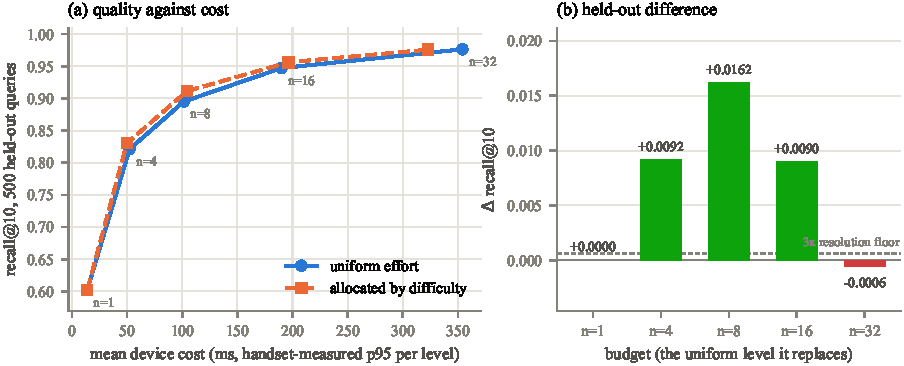
\includegraphics[width=\textwidth]{fig4_c6.pdf}
\caption{Allocation against uniform effort on $500$ held-out queries. (a)
Recall@$10$ against mean device cost, one curve for uniform effort and one
for the allocation, with the uniform level each point replaces marked. (b)
The per-budget difference in recall@$10$, with the value printed above each
bar and the $3\varepsilon$ resolution floor drawn as a dashed line.}
\label{fig:alloc}
\end{figure*}

Three of five budgets improve, by margins of $45$ to $81$ times the
resolution floor of~(\ref{eq:floor}). The two which do not are explained by
the assignment table rather than by chance. At $\nprobe = 1$ the fitted
assignment is $[1,1,1,1,1]$, because there is no cheaper level to move
effort from, and at $\nprobe = 32$ four of the five buckets are already
above $0.95$ recall, so that there is nothing left to buy. Both failures
were predicted by Table~\ref{tab:separation} before the held-out run was
made, which we note because a method whose failure cases are anticipated by
its own diagnostic is in better shape than one whose failures are
discovered afterwards.

\textbf{An honest statement of the cost axis.} The allocation is
constrained to the budget \emph{on the fit half}. The difficulty mix of the
held-out half is not identical, and so the realized cost drifts in both
directions: the allocation spent $4.6\%$ and $8.8\%$ \emph{less} than the
uniform arm at two budgets, and $2.8\%$ and $3.4\%$ \emph{more} at the
other two. The comparison is therefore at \emph{near}-equal cost and not at
exactly equal cost, and we state it that way rather than report only the
budgets at which the drift happens to favour us.

The budget with the largest recall gain is, inconveniently, one at which
the allocation overspent, by $+1.8\%$ recall for $+2.8\%$ time. A reader
entitled to be suspicious of that should compare the alternative way of
buying recall at this operating point. Climbing the uniform curve from
$\nprobe = 8$ to $\nprobe = 16$ costs $+87\%$ latency for $+5.8\%$ recall,
which is $0.067$ percentage points of recall per point of latency, against
$0.66$ for the allocation. Per millisecond the allocation is therefore
roughly an order of magnitude the better trade. It is a favourable exchange
rate and not a free lunch, and we make no stronger claim.

\textbf{Why the gains are small in absolute terms.} The absolute
improvements, between one and two recall points, are modest, and it is
worth saying explicitly why they are bounded, because the bound is
structural rather than a failure of tuning.

The allocation can only move effort between buckets, and cannot create it.
Its maximum possible gain at a budget is therefore the value of the best
redistribution, which is governed by the \emph{convexity} of the recall
curve of each bucket and by how much those curves differ.
Table~\ref{tab:separation} shows the curves converging rapidly: by $\nprobe
= 8$ the spread between hardest and easiest is already down to
$1.25\times$, and above that the easiest three quintiles have almost
nothing left to give up. The method therefore has the most room exactly in
the band in which our results improve, and it is the band which matters on
a phone, tens to low hundreds of milliseconds; but it is a band and not the
whole curve.

We also note what the result is not. It is not a claim that
difficulty-conditioned allocation beats a well-tuned uniform setting by a
wide margin on every corpus. It is a demonstration that a signal the index
already computes is informative enough to beat uniform allocation at
matched device cost, on held-out queries, with every cost taken from a
physical phone. Given that the signal is free, the relevant comparison is
not against a large gain but against zero.

\section{Evaluation of the control layer}
\label{sec:eval}

Section~\ref{sec:alloc} evaluated the difficulty mechanism in isolation.
This section evaluates the surrounding control layer along four further
axes: the budgeted controller against static configuration, context
reduction, joint control, and the storage regime which forced our choice of
cost model. Section~\ref{sec:energy} then reports the energy measurements.

\subsection{Budgeted control against static configuration}
\label{sec:policies}

Table~\ref{tab:policies} and Fig.~\ref{fig:policies} compare three policies
against one latency budget on one interleaved query stream. The budget,
$14.01$~ms, was fixed from the profile table \emph{before} any policy ran,
being the p95 of the median swept level, and so no policy is judged against
a target derived from its own behaviour. The arms are interleaved rather
than run in sequence, so that drift in the state of the machine is shared
rather than assigned to whichever policy ran last.

\begin{table}[!t]
\caption{Three policies against one declared $14.01$~ms budget,
interleaved on the same query stream, $26\,699$ queries in total. The
overhead column is the decision cost of the controller itself as a fraction
of the query it governs.}
\label{tab:policies}
\centering
\begin{tabular}{lrrrrrr}
\toprule
Policy & queries & p50 & p95 & over budget & recall@10 & overhead \\
 & & (ms) & (ms) & & & p95 \\
\midrule
\textsc{Static} & 7\,228  & 11.88 & 14.20 & 5.98\% & \textbf{0.8480} & 0.006\% \\
\textsc{Aimd}   & 8\,790  & 10.07 & 13.44 & 4.31\% & 0.8103 & 0.131\% \\
\textsc{Budget} & 10\,681 & 7.98  & 9.51  & \textbf{0.17\%} & 0.7797 & 0.167\% \\
\bottomrule
\end{tabular}
\end{table}

\begin{figure*}[!t]
\centering
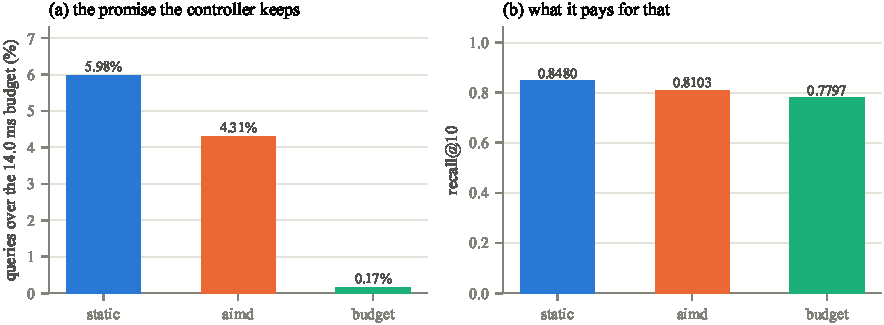
\includegraphics[width=\textwidth]{fig6_policies.pdf}
\caption{The three policies of Table~\ref{tab:policies} on the same
$26\,699$ queries. (a) The percentage of queries which exceeded the
$14.0$~ms budget, one bar per policy. (b) The recall@$10$ of the same three
arms, with the value printed above each bar.}
\label{fig:policies}
\end{figure*}

The budgeted controller reduces deadline misses by $35\times$ and pays
$0.068$ recall for it. We report both numbers because the trade \emph{is}
the result; a paper reporting only the reduction in violations would be
describing half of what happened. The decision of the controller costs at
most $0.167\%$ of the query it governs, and so it is not consuming what it
saves, which is the check any control layer owes its reader, and one which
a learned difficulty classifier would have to pass on the same axis.

\textsc{Aimd} is included because it failed instructively, and not because
it is a strong baseline. It reacts to observed latency, and on a device
whose thermal time constant is $67.9$~s (Section~\ref{sec:method}) a
controller reacting per query is reacting to noise around a slowly moving
mean. It lands between the other two on both axes and is dominated by
neither, which is the signature of a controller adding variance rather than
information. The lesson generalizes beyond our system: the time constant of
the control loop must be matched to the physical process it is controlling,
and on a handset that process is thermal mass and not queue depth.

\subsection{Context reduction is a measured cost and not a free saving}
\label{sec:scr}

We evaluated Selective Content Reduction, which trims retrieved passages
before they reach the generator, on $1\,000$ questions with retrieval held
fixed across the arms by construction, so that any difference is
attributable to the reduction and not to a different set of passages
(Table~\ref{tab:scr}).

\begin{table}[!t]
\caption{Context reduction on $1\,000$ questions, with retrieval identical
across the arms by construction. $\Delta$F1 is against the \textsc{off}
arm, with a paired bootstrap $95\%$ confidence interval.}
\label{tab:scr}
\centering
\begin{tabular}{lrrl}
\toprule
Arm & EM & F1 & $\Delta$F1 (95\% CI) \\
\midrule
\textsc{off}        & 0.6060 & \textbf{0.6769} & --- \\
\textsc{keep1\_ext} & 0.5950 & 0.6661 & $-0.011$ $[-0.021, -0.001]$ \\
\textsc{keep2}      & 0.5850 & 0.6569 & $-0.020$ $[-0.033, -0.008]$ \\
\textsc{keep1}      & 0.5110 & 0.5824 & $-0.095$ $[-0.115, -0.074]$ \\
\bottomrule
\end{tabular}
\end{table}

Every reduction level we tested cost answer quality, and the paired
bootstrap confirms that the losses are significant for all three arms,
since no interval crosses zero. The best configuration is reduction
switched \emph{off}, and that is the default we ship.

This is a negative result for the reduction half of the design. It is worth
contrasting with the positive results recently reported for adaptive
compression on edge RAG~\cite{feric2026adaptivecompression}, which saves
substantial energy at maintained generation quality. We do not read the two
as contradictory. That work compresses adaptively under telemetry guidance,
whereas our arms apply a fixed reduction rule to every question, and a
fixed rule is exactly the uniform-allocation failure mode this paper is
about, transposed to a different stage of the pipeline. The natural reading
of Table~\ref{tab:scr} is that reduction, like retrieval effort, should be
conditioned rather than fixed.

\subsection{Joint control reaches points which neither dimension reaches alone}
\label{sec:joint}

Section~\ref{sec:scr} established that reduction costs quality when it is
applied uniformly. The question this section asks is different: whether, at
a fixed cost ceiling, a joint setting of effort and reduction can reach a
point which neither dimension reaches alone. Sweeping retrieval effort
$\{1,4,16\}$ against reduction
$\{\textsc{off},\textsc{keep2},\textsc{keep1}\}$ on $250$ questions gives
the nine operating points of Table~\ref{tab:joint}. The cost axis is median
retrieval time plus median generation time; the cost of the reduction
itself is excluded and reported separately, because it was measured against
a warm embedding cache, and folding a warm-cache number into the cost axis
would make reduction look nearly free.

\begin{table}[!t]
\caption{A joint sweep of retrieval effort against context reduction, $250$
questions, $k = 5$. Generation is a host number. The cells marked $\star$
sit on the quality/cost Pareto front, in that no single-dimension setting
both matches their F1 and undercuts their cost.}
\label{tab:joint}
\centering
\begin{tabular}{llrrrc}
\toprule
\nprobe & reduction & EM & F1 & cost (ms) & prompt tok. \\
\midrule
1  & \textsc{off}   & 0.476 & 0.5287 & 1021.6 & 572.7 \\
1  & \textsc{keep2} & 0.476 & 0.5256 & 780.9  & 443.0 \\
1  & \textsc{keep1} & 0.420 & 0.4710 & 516.1  & 265.7 $\star$ \\
4  & \textsc{off}   & 0.588 & 0.6459 & 1042.8 & 569.5 \\
4  & \textsc{keep2} & 0.584 & 0.6374 & 804.3  & 444.6 $\star$ \\
4  & \textsc{keep1} & 0.524 & 0.5779 & 525.9  & 268.6 $\star$ \\
16 & \textsc{off}   & 0.648 & \textbf{0.7134} & 1062.8 & 573.7 \\
16 & \textsc{keep2} & 0.640 & 0.7017 & 836.6  & 447.7 \\
16 & \textsc{keep1} & 0.572 & 0.6351 & 550.2  & 269.9 \\
\bottomrule
\end{tabular}
\end{table}

Three of the nine cells sit on the quality/cost Pareto front, meaning that
no single-dimension setting both matches their quality and undercuts their
cost. None dominates the best single-dimension setting outright, and so the
gain is a trade-off along the front rather than a free win, which is the
claim we make and the only claim the data supports. For a system which must
sometimes answer under a hard cost ceiling, reaching three additional
points on the front is a usable result even when none of them dominates.

\subsection{Distance computations are the wrong cost model on a phone}
\label{sec:regime}

Our index stores each cluster as a flat array rather than as the
per-cluster HNSW graph which the EcoVector design
specifies~\cite{park2025mobilerag}. That choice was forced by measurement,
and the measurement bears on how mobile retrieval costs should be modelled
at all.

The search-time analysis of MobileRAG predicts that per-cluster graphs win
provided $\mathit{ef}_L \cdot M' < N/N_c$. We swept both structures inside
that regime ($N/N_c = 4000$), at four operating points chosen to span
recall from $0.65$ to $0.98$. Table~\ref{tab:regime} reports the full
sweep rather than the single matched-recall point we reported previously,
because the pattern is the result.

\begin{table}[!t]
\caption{Per-cluster graphs against flat clusters across a four-point
sweep, inside the regime in which the analytic condition predicts that
graphs win ($N/N_c = 4000$). Each block of three rows is one matched-recall
operating point. The best wall-clock in each block is in bold, as is the
lowest distance count.}
\label{tab:regime}
\centering
\begin{tabular}{lrrr}
\toprule
Cluster storage & recall & dist. comps. & wall-clock (ms) \\
\midrule
flat array      & 0.6507 & 8\,784  & \textbf{8.46}   \\
HNSW, $M{=}16$  & 0.6487 & \textbf{2\,298}  & 22.28  \\
HNSW, $M{=}32$  & 0.6493 & 4\,343  & 29.90  \\
\midrule
flat array      & 0.8197 & 17\,298 & \textbf{112.41} \\
HNSW, $M{=}16$  & 0.8173 & \textbf{4\,346}  & 235.41 \\
HNSW, $M{=}32$  & 0.8183 & 8\,436  & 258.36 \\
\midrule
flat array      & 0.9243 & 34\,071 & \textbf{114.14} \\
HNSW, $M{=}16$  & 0.9220 & \textbf{8\,442}  & 292.52 \\
HNSW, $M{=}32$  & 0.9227 & 16\,625 & 305.54 \\
\midrule
flat array      & 0.9807 & 67\,287 & \textbf{51.93}  \\
HNSW, $M{=}16$  & 0.9783 & \textbf{16\,634} & 138.13 \\
HNSW, $M{=}32$  & 0.9787 & 32\,998 & 143.63 \\
\bottomrule
\end{tabular}
\end{table}

The graphs do what the theory says. At matched recall they cut distance
computations by $3.8\times$ to $4.0\times$ at every point of the sweep.
They also lose on wall-clock at every point of the sweep, by $2.1\times$ to
$2.7\times$. The reason is that the analytic model counts distance
computations and has no term for turning bytes on disk into a searchable
structure, a cost we measured at $95$--$99\%$ of cluster load time. A graph
must be reconstructed before it can be traversed, whereas a flat array can
be scanned where it lies.

We report this not to dispute the arithmetic of the baseline, which is
correct within its own accounting, but to support the methodological
position of Section~\ref{sec:method}. On a phone, a cost model denominated
in distance computations can be internally consistent and still point the
design in the wrong direction, because the dominant term is not in the
model. It is also the concrete reason our controller chooses from a table
of measured latencies rather than from any model, analytic or fitted.

\subsection{Index footprint}

For completeness we report the resident footprint of the index against the
raw vector size on two corpora, since memory is the constraint which
motivates the disk-resident design in the first place. On the NYTimes
corpus the index held $41.0$~MB resident against $283.0$~MB of raw vectors,
and on SIFT1M it held $11.9$~MB against $488.3$~MB. Both are inside the
budgets we declared in advance, $56.6$~MB and $97.7$~MB respectively. We
note in Section~\ref{sec:threats} that the timing samples in that
acceptance run were taken on a machine where $12.4\%$ of samples exceeded
our load threshold; we kept and labelled them rather than silently re-run
until the machine was quiet.

\subsection{Per-query energy, measured}
\label{sec:energy}

Over $9\,670$ queries in $21.0$ minutes on an \emph{unplugged} handset,
with all $218$ telemetry samples reporting \textsc{discharging} and all
currents negative, we integrate $V \cdot I \,\mathrm{d}t$ rather than scale
a current by a nominal voltage. The measured terminal voltage sags from
$4.118$ to $4.058$~V under load, and so the distinction is not academic:
assuming a nominal voltage would bias every figure in the table by a
systematic and load-correlated amount. Table~\ref{tab:energy} summarizes
the run.

\begin{table}[!t]
\caption{Energy measured on the unplugged handset over $9\,670$ queries and
$21.0$ minutes, from $218$ telemetry samples, all of which reported
discharge.}
\label{tab:energy}
\centering
\begin{tabular}{lr}
\toprule
Total energy & $1\,266.6$ J \\
Mean power & $1.006$ W \\
Median power & $0.868$ W \\
Power, 5th--95th percentile & $0.456$--$1.785$ W \\
Measured idle power & $0.657$ W \\
Terminal voltage range & $4.058$--$4.118$ V \\
All-in per query & $130.99$ mJ \\
Marginal cost per cluster opened & $3.21$ mJ \\
\bottomrule
\end{tabular}
\end{table}

\begin{figure}[!t]
\centering
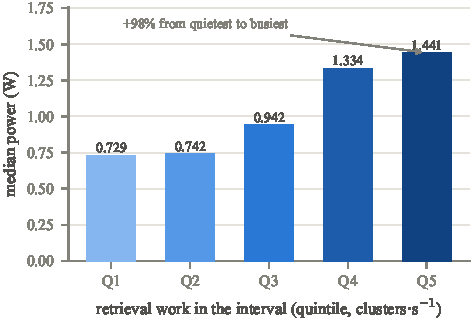
\includegraphics[width=\columnwidth]{fig7_energy.pdf}
\caption{Median power against retrieval work, measured on the unplugged
handset. The intervals of the run are binned into quintiles of retrieval
work rate, in clusters per second, and the median power of each quintile is
printed above its bar. The quintiles are ordered, and so they take one
stepped hue.}
\label{fig:energy}
\end{figure}

Fig.~\ref{fig:energy} shows why retrieval effort is worth controlling at
all. Binning the intervals of the run into quintiles of retrieval work
rate, the median power rises from $0.729$~W in the quietest quintile,
covering $4.7$--$113.8$ clusters$\cdot$s$^{-1}$, to $1.441$~W in the
busiest, covering $161.8$--$202.2$ clusters$\cdot$s$^{-1}$, which is a rise
of $97.6\%$. Had power been flat across effort there would have been
nothing for any policy to save, and this paper would have had no energy
argument to make.

Two caveats belong next to these numbers. First, the all-in figure of
$130.99$~mJ per query divides total energy by query count, and therefore
includes the idle draw of the device; the measured idle power of $0.657$~W
accounts for roughly three-quarters of median power, which is why the
\emph{marginal} figure of $3.21$~mJ per cluster is the one a controller can
act on. Second, the regression behind that marginal figure explains $R^2 =
0.16$ of the variance in interval power. That is low, and it is the honest
figure, since most of the power draw of a phone during a retrieval workload
is not retrieval. We report it rather than report only the slope, because a
slope without its $R^2$ invites the reader to assume a tighter relation
than we observed.

\section{A negative result: the shield reads the wrong thermometer}
\label{sec:sensors}

\textbf{The policy, and what it did.} We built a device-state policy which
derates retrieval effort on thermal and battery grounds, with a warm
threshold at $42\degC$ and a hot threshold at $46\degC$. The thresholds
were not round numbers chosen for tidiness. They were anchored on the one
thermal measurement we had when we wrote the policy: the skin sensor of the
handset sat at $36.6\degC$ idle and reached $41.4\degC$ after $60$~s of
full load, and so $42\degC$ was calibrated to mean sustained load beyond
anything we had observed in a burst.

Run on the handset over $22.0$ minutes and $19\,719$ decisions per arm, the
policy looks like a success on latency. It cut p95 from $84.7$ to
$43.3$~ms and deadline misses from $1.11\%$ to $0.01\%$, at a cost of
$0.10$ recall. Reported on its own, that is a publishable-looking table.

It is also not evidence for a thermal policy. Only $542$ of the $19\,719$
decisions, which is $2.7\%$, had any device signal behind them at all. The
other $97.3\%$ were taken blind and reduce exactly to the budgeted policy
of Section~\ref{sec:policies}. The latency improvement is real and it
belongs to the budgeted controller and not to the shield. This is the point
at which the \texttt{NaN} discipline of Section~\ref{sec:method} earned its
cost. An implementation defaulting to zero would have recorded $19\,719$
decisions taken at a comfortable $0\degC$ and reported a thermal policy
which worked.

\textbf{Why.} Fig.~\ref{fig:sensors} shows the cause, across every run we
recorded and not only the one which happened to illustrate it. Android
exposes a skin temperature intended to model what a hand feels, and
separately exposes per-zone sensors reporting individual components. On all
six runs the skin sensor peaked between $34.0$ and $37.5\degC$ while the
hottest zone peaked between $54.1$ and $78.8\degC$, a divergence of $20.1$
to $41.3\degC$, in the same device, during the same workload, at the same
instant.

\begin{figure}[!t]
\centering
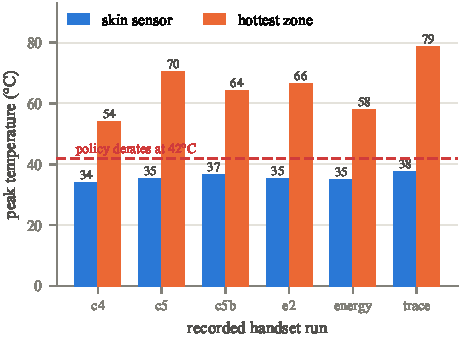
\includegraphics[width=\columnwidth]{fig5_sensors.pdf}
\caption{Peak temperature per recorded handset run, by sensor. Each run
contributes one pair of bars, the skin sensor and the hottest internal
zone, with the peak printed above each bar. The dashed line is the $42\degC$
threshold at which the policy derates.}
\label{fig:sensors}
\end{figure}

The consequence is stark and it is reproducible. Fig.~\ref{fig:trace}
replays one recorded run through the same policy, changing only which
sensor the policy reads. Reading the skin, the threshold is never crossed
and the controller spends $97\%$ of the run at full effort. Reading the
hottest zone, it derates across $100\%$ of the run, all the way down to the
floor level, giving up $0.266$ recall against what the latency budget alone
would have allowed. Same policy, same code path, same trace, same
thresholds, and opposite behaviour.

\begin{figure}[!t]
\centering
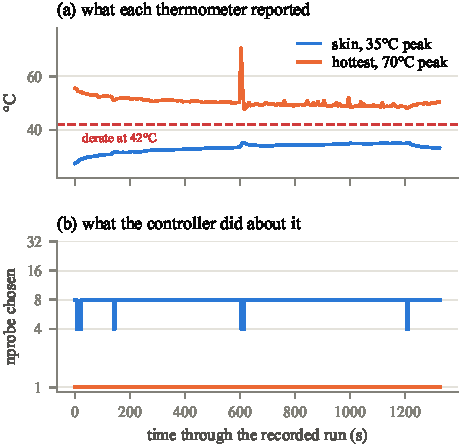
\includegraphics[width=\columnwidth]{fig8_trace.pdf}
\caption{One recorded run, one policy, two thermometers. (a) The two sensor
traces through the run, with the $42\degC$ derate threshold drawn as a
dashed line. (b) The \nprobe{} the controller chose at each point of the
run under each sensor.}
\label{fig:trace}
\end{figure}

\textbf{What we take from it.} Neither sensor is obviously the correct one,
which is what makes this a design problem rather than a bug. The skin
sensor is the right quantity for user comfort, is what a vendor intends a
thermal policy to read, and is the one exposed through the stable platform
API. The hottest zone is the right quantity for component stress, but it is
a spike-prone signal which, at our thresholds, would derate a retrieval
system almost permanently under any sustained workload; and a shield which
is always engaged is not a shield, it is a lower performance ceiling.

Our policy is therefore not so much miscalibrated as pointed at a signal
which does not carry the information the shield needs at the threshold at
which the shield acts. The specific failure has three parts, and each is
worth stating separately because each is independently avoidable.

\begin{enumerate}
\item \emph{Calibrating on a burst.} The thresholds came from a $60$~s
full-load measurement. The thermal time constant of the device is
$67.9$~s, and so a $60$~s burst observes less than one time constant of the
process it is supposed to characterize.
\item \emph{Assuming one device temperature.} There is no such quantity. A
handset under load has a temperature field, and the two scalars the
platform exposes sit at opposite ends of it.
\item \emph{Validating the policy on latency.} The policy was first
evaluated by whether it hit its latency target, which it did, for reasons
which had nothing to do with its thermal logic.
\end{enumerate}

A practitioner building a thermally-aware mobile system should therefore
measure \emph{both} sensors on the target device before choosing
thresholds, should expect them to disagree by tens of degrees, should
calibrate on runs at least several time constants long, and should
instrument how many control decisions actually had a signal behind them.
Recent thermal-aware inference systems~\cite{zou2026enerinfer,lu2026therme}
take a thermal observable as given and build sophisticated prediction on top
of it. Our result suggests that the observable itself deserves a validation
step, and that a system reporting thermal-policy success should report what
fraction of its decisions were informed.

We publish this because it is the kind of result which is expensive to
rediscover and cheap to share, and because the apparatus which produced our
positive results is the same apparatus which produced this one.

\section{Discussion}
\label{sec:discussion}

\textbf{When does the method transfer?} The mechanism requires four
conditions, and we state them as conditions rather than as assumptions
because each is checkable on a candidate deployment before any code is
written.

\emph{A two-phase index.} There must be a cheap phase whose output is
available before an expensive phase commits. IVF-style and
centroid-plus-disk designs qualify; DiskANN~\cite{subramanya2019diskann},
SPANN~\cite{chen2021spann}, EcoVector~\cite{park2025mobilerag} and
EdgeRAG~\cite{seemakhupt2024edgerag} all have the shape. A flat scan or a
single-level graph does not.

\emph{An asymmetric cost--recall curve.} If effort bought recall linearly,
reallocation would gain nothing. Table~\ref{tab:profile} shows a factor of
$31$ between the recall per millisecond of the first step and of the last
on our index, and we would expect a method deployed on a near-linear curve
to produce differences near the resolution floor.

\emph{A difficulty signal which separates.} Table~\ref{tab:separation} is
the diagnostic, and it can be produced offline from a recall sweep before
anything is deployed. If the quintiles do not separate at the cheapest
level then the method has nothing to work with, and the practitioner finds
that out for the cost of one sweep.

\emph{Costs measured on the target.} Section~\ref{sec:regime} is the
cautionary case. Had we populated $c_\ell$ from the analytic model, we
would have chosen per-cluster graphs and been slower by a factor of $2.6$
while believing we were faster by a factor of $4$.

\textbf{Composition with other adaptive mechanisms.} Nothing in this design
competes with the adjacent mechanisms, and the interesting question is how
they stack. A strategy-level router such as
Adaptive-RAG~\cite{jeong2024adaptiverag} decides \emph{whether} to
retrieve; our controller decides \emph{how hard} to retrieve, for the
queries which survive that decision; and an early-termination rule such as
DARTH~\cite{chatzakis2026darth} could then decide when to stop inside the
budget we set. The three act at different times and read different signals,
and we see no interaction which would make them incompatible. A
telemetry-guided compressor~\cite{feric2026adaptivecompression} acts after
all three, on the context handed to the generator, and
Section~\ref{sec:joint} is a first measurement of what that composition
buys and costs.

The ordering matters, for a reason worth stating. Our signal is available
earliest of the four, before any cluster is opened, which means that it is
the only one of them which can prevent work rather than abandon it. On a
device where the dominant cost is loading bytes and reconstructing
structures (Section~\ref{sec:regime}), preventing work and abandoning work
are not equivalent.

\textbf{Implications for index designers.} Two implications follow for
anyone building a mobile vector index, and neither requires adopting our
controller.

First, the probe phase should expose its distances and not only its
ranking. In our implementation they were already computed and then
discarded at the API boundary. Any index which returns only cluster
identifiers has thrown away a free difficulty signal, and restoring it
costs nothing but a wider return type.

Second, a profile table should be a first-class artifact of the index,
built on the target device at install or at first run and stored alongside
it. Our controller reads five rows; producing them took minutes of device
time and removed every dependence on a cost model. Given
Section~\ref{sec:regime}, in which a correct analytic model pointed the
design in the wrong direction, we would argue that the profile table is the
more defensible foundation even for systems which do not adapt per query.

\section{Threats to validity}
\label{sec:threats}

\textbf{Construct validity.} \emph{Recall@$10$ is a proxy for answer
quality.} The allocation optimizes retrieval recall and not end-to-end
answer correctness. Section~\ref{sec:joint} measures EM and F1 and shows
them moving with retrieval effort as expected, but the allocation itself
was never optimized against F1. A gain of one to two recall points need not
produce a proportional gain in answer quality, and we do not claim that it
does.

\emph{Cost is p95 latency from a table.} The notion of cost the controller
has is the measured p95 of a level, which is a population statistic rather
than a property of the individual query it is about to run. This is
deliberate, since a per-query cost prediction is exactly the model we
discarded in Section~\ref{sec:design}, but it does mean the budget is
honoured in expectation and not per query.

\textbf{Internal validity.} \emph{The generation stage is a host number.}
Retrieval, its latency and its energy were measured on the device.
\texttt{flan-t5-base} generation was run on a host, and every generation
timing in this paper is labelled as such. An end-to-end on-device latency
figure would require a quantized generator and is future work. This affects
Table~\ref{tab:joint} in particular, whose cost axis is dominated by the
host generation term.

\emph{The footprint acceptance run was contended.} The timing samples in
that run were taken with $12.4\%$ of samples above our declared load
threshold. We kept and labelled them rather than silently re-run until the
machine was quiet, but the resulting timings should be read as upper
bounds.

\emph{The thermal decomposition is refused and not merely uncertain.} We
can say what fraction of measured \emph{power} retrieval accounts for,
$29.9\%$ on one trace, but we cannot decompose a temperature rise, for the
reason given in Section~\ref{sec:method}, and we decline to report a number
we do not trust.

\textbf{External validity.} \emph{One device and one corpus for the main
result.} The profile table, the energy measurements and the thermal runs
are all from a single handset model (vivo I2304), and the allocation is
fitted on one corpus. Difficulty buckets are a property of the cluster
geometry of a particular index, and we deliberately refuse to load a fit
across corpora for that reason. Generality across devices and corpora is
unestablished, and establishing it is the first item of future work.

\emph{The policy comparison uses a different corpus.}
Section~\ref{sec:policies} is on SIFT1M, whereas the profile table and the
allocation are on SQuAD. The two are not directly comparable and we do not
combine them anywhere.

\emph{The storage comparison is one index configuration.} Our clusters
average $216$ vectors. Per-cluster graphs may well pay at cluster sizes
large enough to amortize the cost of constructing them; our result is that
they do not at the sizes this design produces, inside the regime in which
the analytic condition predicts that they should.

\emph{The monotonicity of Table~\ref{tab:separation} is observed and not
proven.} We rely on recall being monotone in the bucket index and on the
marginal gain being anti-monotone. Both hold with no inversions across all
$25$ cells on this index and this corpus. Neither is guaranteed by the
geometry, and a corpus with strongly anisotropic clusters could violate
them; the diagnostic of Section~\ref{sec:discussion} would detect that
before deployment.

\section{Reproducibility}
\label{sec:repro}

All experiments are reproducible from the released repository. The design
rules the artifact follows are the ones stated in Section~\ref{sec:method},
and they are enforced mechanically rather than by convention.

\begin{itemize}
\item Every figure and table in this paper is generated by a script which
reads a JSON or Parquet file written by a recorded run. No number is typed
into the manuscript by hand.
\item A checking script asserts the figures of the manuscript against the
recorded results and fails if any has drifted. It caught two errors while
this manuscript was being written.
\item The expensive measurement underlying Section~\ref{sec:alloc} is
cached, so that the allocation and its verdict can be re-derived in seconds
from identical numbers rather than by re-running the sweep.
\item The seed governing the fit/test split is fixed and is recorded in the
results file alongside the numbers it produced.
\item An end-to-end verification harness re-runs every acceptance gate,
including the test suite, the linters and the type checker, and records the
exit status of each.
\end{itemize}

Device telemetry traces are released in the form in which they were
recorded, as line-delimited JSON, including the runs in which a sensor was
unavailable, so that the $97.3\%$ figure of Section~\ref{sec:sensors} can
be recomputed rather than taken on trust.

\section{Conclusion and open questions}
\label{sec:conclusion}

A two-phase on-device vector index computes, for free, a signal which
predicts how much effort each query needs, and until now that signal was
discarded at the API boundary. We showed that it separates recall@$10$ at
the cheapest effort level by $3.5\times$ across difficulty quintiles, and
that the marginal value of one step of effort differs by $45\times$ between
the hardest and the easiest fifth of queries. We fitted an allocation
against costs measured on a physical handset, solved it exactly, and
validated on held-out queries that it beats uniform allocation at
near-equal device cost on three of five budgets, buying recall per
millisecond roughly an order of magnitude more efficiently than climbing
the uniform curve does.

We also showed a thermal shield failing for a reason worth publishing. The
sensor which a mobile platform makes conventional never reaches the
threshold at which the shield is calibrated to act, while an internal zone
on the same device exceeds it on every recorded run, and the choice between
them changes the behaviour of the controller completely. We report that
failure using the same apparatus which produced our positive results, which
is the point of building the apparatus.

Four questions follow directly. The first and most important concerns
generality: the same diagnostic applied across devices and corpora would
establish whether the separation we measure is a property of this index or
of the family. A natural second question is whether composition with early
termination works as cleanly as it appears it should, combining a budget
chosen before search with a stopping rule evaluated during it, since the
two mechanisms read disjoint signals. A third is whether a continuous
allocation, replacing the bucketed table with a monotone function of $g$,
is worth the exactness of enumeration it would trade away. And it remains
open whether an energy-denominated budget, substituting the measured
marginal $3.21$~mJ per cluster for milliseconds in the constraint
of~(\ref{eq:alloc}), behaves like the latency-denominated one; our
measurements already support the substitution, and it is the budget a user
actually cares about on a device which will not charge until evening.

\section*{Acknowledgment}

The authors thank the reviewers whose questions sharpened the statement of
the cost axis in Section~\ref{sec:alloc}, and record that the negative
result of Section~\ref{sec:sensors} survived into this paper because the
measurement apparatus made it impossible to overlook.

\begin{thebibliography}{00}

\bibitem{lewis2020rag}
P.~Lewis \emph{et al.}, ``Retrieval-augmented generation for
knowledge-intensive NLP tasks,'' in \emph{Advances in Neural Information
Processing Systems}, vol.~33, 2020, pp.~9459--9474.

\bibitem{park2025mobilerag}
J.~Park, S.~Lee, and H.~Kim, ``MobileRAG: Enabling efficient
retrieval-augmented generation on mobile devices,'' arXiv:2507.01079, 2025.

\bibitem{malkov2020hnsw}
Y.~A. Malkov and D.~A. Yashunin, ``Efficient and robust approximate nearest
neighbor search using hierarchical navigable small world graphs,'' \emph{IEEE
Trans. Pattern Anal. Mach. Intell.}, vol.~42, no.~4, pp.~824--836, 2020.

\bibitem{johnson2021faiss}
J.~Johnson, M.~Douze, and H.~J\'egou, ``Billion-scale similarity search with
GPUs,'' \emph{IEEE Trans. Big Data}, vol.~7, no.~3, pp.~535--547, 2021.

\bibitem{douze2024faiss}
M.~Douze \emph{et al.}, ``The Faiss library,'' arXiv:2401.08281, 2024.

\bibitem{subramanya2019diskann}
S.~J. Subramanya, F.~Devvrit, H.~V. Simhadri, R.~Krishnaswamy, and
R.~Kadekodi, ``DiskANN: Fast accurate billion-point nearest neighbor search on
a single node,'' in \emph{Advances in Neural Information Processing Systems},
vol.~32, 2019.

\bibitem{li2020earlytermination}
C.~Li, M.~Zhang, D.~G. Andersen, and Y.~He, ``Improving approximate nearest
neighbor search through learned adaptive early termination,'' in \emph{Proc.
ACM SIGMOD Int. Conf. Management of Data}, 2020, pp.~2539--2554.

\bibitem{guo2020scann}
R.~Guo, P.~Sun, E.~Lindgren, Q.~Geng, D.~Simcha, F.~Chern, and S.~Kumar,
``Accelerating large-scale inference with anisotropic vector quantization,''
in \emph{Proc. Int. Conf. Machine Learning}, 2020, pp.~3887--3896.

\bibitem{rajpurkar2016squad}
P.~Rajpurkar, J.~Zhang, K.~Lopyrev, and P.~Liang, ``SQuAD: 100,000+ questions
for machine comprehension of text,'' in \emph{Proc. Conf. Empirical Methods in
Natural Language Processing}, 2016, pp.~2383--2392.

\bibitem{chung2024flan}
H.~W. Chung \emph{et al.}, ``Scaling instruction-finetuned language models,''
\emph{J. Mach. Learn. Res.}, vol.~25, no.~70, pp.~1--53, 2024.

\bibitem{jeong2024adaptiverag}
S.~Jeong, J.~Baek, S.~Cho, S.~J. Hwang, and J.~C. Park, ``Adaptive-RAG:
Learning to adapt retrieval-augmented large language models through question
complexity,'' in \emph{Proc. NAACL-HLT}, 2024, pp.~7036--7050.

\bibitem{asai2024selfrag}
A.~Asai, Z.~Wu, Y.~Wang, A.~Sil, and H.~Hajishirzi, ``Self-RAG: Learning to
retrieve, generate, and critique through self-reflection,'' in \emph{Proc.
Int. Conf. Learning Representations}, 2024.

\bibitem{jiang2023flare}
Z.~Jiang, F.~F. Xu, L.~Gao, Z.~Sun, Q.~Liu, J.~Dwivedi-Yu, Y.~Yang, J.~Callan,
and G.~Neubig, ``Active retrieval augmented generation,'' in \emph{Proc. Conf.
Empirical Methods in Natural Language Processing}, 2023, pp.~7969--7992.

\bibitem{mallen2023whennot}
A.~Mallen, A.~Asai, V.~Zhong, R.~Das, D.~Khashabi, and H.~Hajishirzi, ``When
not to trust language models: Investigating effectiveness of parametric and
non-parametric memories,'' in \emph{Proc. Annu. Meeting Assoc. Computational
Linguistics}, 2023, pp.~9802--9822.

\bibitem{seemakhupt2024edgerag}
K.~Seemakhupt, S.~Liu, and S.~Khan, ``EdgeRAG: Online-indexed RAG for edge
devices,'' arXiv:2412.21023, 2024.

\bibitem{chatzakis2026darth}
M.~Chatzakis, Y.~Papakonstantinou, and T.~Palpanas, ``DARTH: Declarative
recall through early termination for approximate nearest neighbor search,'' in
\emph{Proc. ACM SIGMOD Int. Conf. Management of Data}, 2026.
(arXiv:2505.19001)

\bibitem{chen2021spann}
Q.~Chen, B.~Zhao, H.~Wang, M.~Li, C.~Liu, Z.~Li, M.~Yang, and J.~Wang,
``SPANN: Highly-efficient billion-scale approximate nearest neighbor search,''
in \emph{Advances in Neural Information Processing Systems}, vol.~34, 2021.

\bibitem{aumuller2020annbench}
M.~Aum\"uller, E.~Bernhardsson, and A.~Faithfull, ``ANN-Benchmarks: A
benchmarking tool for approximate nearest neighbor algorithms,'' \emph{Inf.
Syst.}, vol.~87, Art.~101374, 2020.

\bibitem{karpukhin2020dpr}
V.~Karpukhin, B.~O\u{g}uz, S.~Min, P.~Lewis, L.~Wu, S.~Edunov, D.~Chen, and
W.~Yih, ``Dense passage retrieval for open-domain question answering,'' in
\emph{Proc. Conf. Empirical Methods in Natural Language Processing}, 2020,
pp.~6769--6781.

\bibitem{li2023gte}
Z.~Li, X.~Zhang, Y.~Zhang, D.~Long, P.~Xie, and M.~Zhang, ``Towards general
text embeddings with multi-stage contrastive learning,'' arXiv:2308.03281,
2023.

\bibitem{gao2023ragsurvey}
Y.~Gao \emph{et al.}, ``Retrieval-augmented generation for large language
models: A survey,'' arXiv:2312.10997, 2023.

\bibitem{laskaridis2024melt}
S.~Laskaridis, K.~Katevas, L.~Minto, and H.~Haddadi, ``MELTing point: Mobile
evaluation of language transformers,'' in \emph{Proc. ACM Int. Conf. Mobile
Computing and Networking}, 2024.

\bibitem{ignatov2019aibench}
A.~Ignatov \emph{et al.}, ``AI benchmark: All about deep learning on
smartphones in 2019,'' in \emph{Proc. IEEE/CVF Int. Conf. Computer Vision
Workshops}, 2019, pp.~3617--3635.

\bibitem{strubell2019energy}
E.~Strubell, A.~Ganesh, and A.~McCallum, ``Energy and policy considerations
for deep learning in NLP,'' in \emph{Proc. Annu. Meeting Assoc. Computational
Linguistics}, 2019, pp.~3645--3650.

\bibitem{schwartz2020greenai}
R.~Schwartz, J.~Dodge, N.~A. Smith, and O.~Etzioni, ``Green AI,''
\emph{Commun. ACM}, vol.~63, no.~12, pp.~54--63, 2020.

\bibitem{wang2025leann}
Y.~Wang, Z.~Li, S.~Liu, Y.~Wu, Z.~Mao, Y.~Zhao, X.~Yan, Z.~Xu, Y.~Zhou,
I.~Stoica, S.~Min, M.~Zaharia, and J.~E. Gonzalez, ``LEANN: A low-storage
vector index,'' arXiv:2506.08276, 2025.

\bibitem{mohoney2025quake}
J.~Mohoney, D.~Sarda, M.~Tang, S.~R. Chowdhury, A.~Pacaci, I.~F. Ilyas,
T.~Rekatsinas, and S.~Venkataraman, ``Quake: Adaptive indexing for vector
search,'' arXiv:2506.03437, 2025.

\bibitem{senkevich2025kscann}
O.~Senkevich \emph{et al.}, ``KScaNN: Scalable approximate nearest neighbor
search on Kunpeng,'' arXiv:2511.03298, 2025.

\bibitem{hua2026hardness}
Z.~Hua, Q.~Mo, Z.~Yao, L.~Cui, X.~Liu, G.~Wang, Z.~Wei, X.~Liu, T.~Tang,
S.~Liu, and L.~Qu, ``Dynamically detect and fix hardness for efficient
approximate nearest neighbor search,'' in \emph{Proc. ACM SIGMOD Int. Conf.
Management of Data}, 2026. (arXiv:2510.22316)

\bibitem{killingback2026unified}
J.~Killingback, O.~Meshi, H.~Li, H.~Zamani, and M.~Karimzadehgan, ``A unified
model and document representation for on-device retrieval-augmented
generation,'' arXiv:2604.14403, 2026.

\bibitem{liu2026percache}
K.~Liu, L.~Zeng, L.~Xu, B.~Yang, and Z.~Yan, ``PerCache: Predictive
hierarchical cache for RAG applications on mobile devices,''
arXiv:2601.11553, 2026.

\bibitem{feric2026adaptivecompression}
Z.~Feric, A.~Taherin, Y.~Wang, and D.~Kaeli, ``From retrieved context to
runtime control: Adaptive compression for edge-based RAG,'' in \emph{Proc. ACM
AI Leadership Summit}, 2026. (arXiv:2608.19535)

\bibitem{ren2024mec}
R.~Ren, Y.~Wu, X.~Zhang, J.~Ren, Y.~Shen, S.~Wang, and K.-F. Tsang,
``Retrieval-augmented generation for mobile edge computing via large language
model,'' arXiv:2412.20820, 2024.

\bibitem{loo2025mobileagent}
G.~Loo, C.~Liu, Q.~Yin, X.~Chen, J.~Chen, J.~Zhang, and Y.~Tian, ``MobileRAG:
Enhancing mobile agent with retrieval-augmented generation,''
arXiv:2509.03891, 2025.

\bibitem{zou2026enerinfer}
B.~Zou, N.~Liu, B.~Sun, M.~Mascherin, D.~Roy, Y.~Liu, Y.~Peng, N.~Jia, and
H.~Chen, ``EnerInfer: Energy-aware on-device LLM inference,''
arXiv:2606.23001, 2026.

\bibitem{lu2026therme}
R.~Lu, Y.~Wang, and B.~Liu, ``ThermE: Predictive management of shared thermal
headroom for sustained LLM inference on thermally constrained edge SoCs,''
arXiv:2610.00267, 2026.

\bibitem{tummalapalli2026edgeinference}
P.~Tummalapalli, S.~Arayakandy, R.~Pal, and K.~Kundan, ``LLM inference at the
edge: Mobile, NPU, and GPU performance efficiency trade-offs under sustained
load,'' arXiv:2603.23640, 2026.

\bibitem{cai2026npuready}
G.~Cai, R.~Tian, L.~Yang, Z.~Ren, J.~Yuan, L.~Li, and J.~Wang, ``Is your NPU
ready for LLMs? Dissecting the hidden efficiency bottlenecks in mobile LLM
inference,'' arXiv:2607.05475, 2026.

\bibitem{ehsani2026sustainability}
E.~Ehsani, L.~Giamattei, I.~Malavolta, and R.~Pietrantuono, ``Sustainability
is not linear: Quantifying performance, energy, and privacy trade-offs in
on-device intelligence,'' arXiv:2603.26603, 2026.

\end{thebibliography}

\end{document}
